\documentclass[a4paper]{article}

\usepackage[utf8]{inputenc}
\usepackage[spanish]{babel}
\usepackage{float}
\usepackage{fancyhdr,graphicx,listings,amsmath}
\usepackage[colorlinks=true,linkcolor=black,urlcolor=blue,bookmarksopen=true]{hyperref}

\newcommand{\materia}{[75.06 / 95.58] Organización de Datos}
\newcommand{\trabajo}{Trabajo Práctico 1: Análisis Exploratorio de Datos}
\newcommand{\trabajoheader}{TP1}
\newcommand{\cuatri}{2c2018}
\newcommand{\cuatrimestre}{Segundo cuatrimestre de 2018}
\newcommand{\grupo}{Grupo Datatouille}
\newcommand{\repo}{https://github.com/FdelMazo/7506-Datos/}
\newcommand{\kernel}{https://kaggle.com/datatouille2018/7506-TP1/}
\newcommand{\alumnos}{
    del Mazo, Federico & 100029 & delmazofederico@gmail.com\\
    Bojman, Camila & 101055 &  camiboj@gmail.com\\
    Hortas, Cecilia & 100687 & ceci.hortas@gmail.com\\
    Souto, Rodrigo & 97649 & rnsoutob@gmail.com\\
}
\newcommand{\curso}{Curso 01}
\newcommand{\docentes}{
    \item Argerich, Luis Argerich
    \item Golmar, Natalia
    \item Martinelli, Damina Ariel
    \item Ramos Mejia, Martín Gabriel
}

\hypersetup{
    pdftitle={\trabajo},
	pdfsubject={\materia},
	pdfauthor={\grupo},
}

\pagestyle{fancy}
\fancyhf{}
\fancyhead[L]{\materia}
\fancyhead[R]{\trabajoheader - \cuatri}
\renewcommand{\headrulewidth}{0.4pt}
\fancyfoot[C]{\thepage}
\renewcommand{\footrulewidth}{0.4pt}

\begin{document}
\pagenumbering{gobble}

\begin{titlepage}
	\hfill
\includegraphics[width=6cm]{fiuba.jpg}
    \begin{center}
    \vfill
    \Huge \textbf{\trabajo}
    \vskip2cm
    \Large \materia\\
    \cuatrimestre
    \vfill
    \begin{flushleft} 
    \grupo
    \end{flushleft}
    \begin{tabular}{|l|c|r|}
	\hline
	Alumno & Padrón & Mail\\
	\hline \hline
    \alumnos
	\hline
	\end{tabular}
    \begin{flushleft} 
    \url{\repo} \\
    \url{\kernel}
    \end{flushleft}
    \vskip1cm
    \end{center}
    \curso
    \begin{itemize}
        \docentes
    \end{itemize}
\end{titlepage}
\pagenumbering{roman}
\tableofcontents
\newpage
\pagenumbering{arabic}
\setcounter{page}{1}

\section{Introducción}

Se propone analizar en el presente informe los datos obtenidos de usuarios que visitaron \texttt{www.trocafone.com}, un sitio de e-commerce de compra y venta de celulares reacondicionados, con operaciones principalmente en Brasil. Para ello, la empresa Trocafone nos proporcionó acceso a los datos a través del archivo \texttt{events.csv}. Estos datos corresponden al período de tiempo comprendido entre el 1 de enero del 2018 al 16 de junio del 2018.

El objetivo de este informe es realizar un análisis de dicho set de datos para obtener un listado de \textit{insights} aprendidos sobre los mismos. Se propone específicamente:
 
 \begin{itemize}
	 \item Descubrir features en el campo \texttt{model}
	 \item Identificar patrones de usuarios que realizan checkouts y conversiones
	 \item Analizar las búsquedas que realizan los usuarios y las \textit{keywords} utilizadas
	 \item Analizar los distintos lugares de dónde se originan las visitas a Trocafone
	 \item Descubrir features jerarquizando alguno de los campos disponibles
	 \item \textbf{agregar más items a medida que desarrollamos el informe}
\end{itemize}

Finalmente se busca realizar un aporte a la empresa Trocafone con datos que sirvan para mejorar sus servicios. 

\section{Información general sobre los datos}

En el archivo proporcionado por la empresa Trocafone se observan las siguientes columnas:

\begin{itemize}
	\item \textbf{timestamp}: Fecha y hora cuando ocurrió el evento.
	\item \textbf{event}: Tipo de evento.
	\item \textbf{person}: Identificador de cliente que realizó el evento.
	\item \textbf{url}: Url visitada por el usuario.
	\item \textbf{sku}: Identificador de producto relacionado al evento.
	\item \textbf{model}: Nombre descriptivo del producto incluyendo marca y modelo.
	\item \textbf{condition}: Condición de venta del producto.
	\item \textbf{storage}: Cantidad de almacenamiento del producto.
	\item \textbf{color}: Color del producto.	
	\item \textbf{skus}: Identificadores de productos visualizados en el evento.
	\item \textbf{search\_term}: Téŕminos de búsqueda utilizados en el evento.
	\item \textbf{static\_page}: Identificador de página estática visitada.
	\item \textbf{campagn\_source}: Origen de campaña, si el tráfico se originó de una campaña de marketing.
	\item \textbf{text\_engine}: Motor de búsqueda desde donde se originó el evento, si aplica.
	\item \textbf{channel}: Tipo de canal desde donde se originó el evento.
	\item \textbf{new\_vs\_returning}: Indicador de si el evento fue generado por un usuario nuevo (New) o por un usuario que previamente había visitado el sitio (Returning) según el motor de analytics.
	\item \textbf{city}: Ciudad desde donde se originó el evento.
	\item \textbf{region}: Región desde donde se originó el evento.
	\item \textbf{country}: País desde donde se originó el evento.
	\item \textbf{device\_type}: Tipo de dispositivo desde donde se genero el evento.
	\item \textbf{screen\_resolution}: Resolución de pantalla que se está utilizando en el dispositivo desde donde se generó el evento.
	\item \textbf{operating\_system\_version}: Versión de sistema operativo desde donde se originó el evento.
	\item \textbf{browser\_version}: Versión del browser utilizado en el evento.
\end{itemize}

\section{Datasets adicionales incoporados para el análisis}

Se utilizan adicionalmente los siguientes archivos para realizar el análisis:

\begin{itemize}
	\item {Mapas de Brazil y Estados unidos: Sacados de Geonames \footnote{\url{http://www.geonames.org/}} }
	\item \texttt{brands.csv} para extraer información del modelo
	\footnote{Detallado en \texttt{anexo.ipynb}}
	\item \texttt{os.csv} para extraer información del sistema operativo
	\footnote{Detallado en \texttt{anexo.ipynb}}
    \item \texttt{browsers.csv} para extraer información de la versión del browser
	\footnote{Detallado en \texttt{anexo.ipynb}}
\end{itemize}


\section{Ejecución}

El trabajo fue realizado en Anaconda \footnote{\url{https://anaconda.org/}}. Para poder replicar el trabajo, hay que también instalar las siguientes librerías adicionales:

\begin{itemize}
	\item{Squarify \footnote{\url{https://github.com/laserson/squarify}}: Para los treemaps.}
	\item{Geopandas \footnote{\url{http://geopandas.org/}}: Para poder graficar sobre mapas geográficos.}
	\item{Wordcloud \footnote{\url{https://github.com/amueller/word_cloud/}}: Para poder visualizar los términos más buscados.}
\end{itemize}

Estos pueden ser instalados con los siguientes comandos: 
\begin{lstlisting}[language=sh]
pip install squarify
conda install -c conda-forge geopandas
conda install -c conda-forge wordcloud
\end{lstlisting}

\section{Análisis de eventos}

En esta sección se propone analizar los distintos tipos de eventos realizados por los usuarios de Trocafone. 

El campo \texttt{event} puede adquirir distintos tipos de valores categóricos que se describen como sigue:

\begin{itemize}
	\item \textbf{"viewed product"}: El usuario visita una página de producto.
	\item \textbf{"brand listing"}: El usuario visita un listado específico de una marca viendo un conjunto de productos.
	\item \textbf{"visited site"}:  El usuario ingresa al sitio a una determinada url.
	\item \textbf{"ad campaign hit"}: El usuario ingresa al sitio mediante una campana de marketing online.
	\item \textbf{"generic listing"}: El usuario visita la homepage.
	\item \textbf{"searched products"}: El usuario realiza una búsqueda de productos en la interfaz de búsqueda del site.
	\item \textbf{"search engine hit"}: El usuario ingresa al sitio mediante un motor de búsqueda web.
	\item \textbf{"checkout"}: El usuario ingresa al checkout de compra de un producto.
	\item \textbf{"static page"}:  El usuario visita una página.
	\item \textbf{"conversion"}: El usuario realiza una conversión, comprando un producto.
	\item \textbf{"lead"}: El usuario se registra para recibir una notificación de disponibilidad de stock, para un producto que no se encontraba disponible en ese momento.					
\end{itemize}

\subsection{Hipótesis sobre el truncamiento de los datos}

Se sabe por información de la consigna que el dataset proporcionado no representa el conjunto total de datos de todos los eventos realizados por los usuarios en el período de tiempo determinado. Es por esta razón que se busca elaborar una hipótesis en base al criterio con el que se fijó la selección de los datos. A partir de un análisis de los mismos se observó que todos los usuarios registrados en el dataset realizaron al menos 1 checkout, por lo que la base de datos original se truncó. Sin ir más lejos es evidente que no todos los usuarios que ingresan al sitio de Trocafone van a realizar un checkout.

De esta manera es importante remarcar que las conclusiones a las que se llegará en el desarrollo del Trabajo Práctico se basan en un sector segmentado de los datos, por lo que en ciertos aspectos del análisis no se podrá arribar a conclusiones fundadas.

\subsection{Conversion rate}

En primer lugar se analiza la llamada \textit{conversion rate} o tasa de conversión debido a su importancia en cualquier negocio de e-commerce.

La tasa de conversión es el porcentaje de visitantes que completan un objetivo deseado (en este caso realizar una conversión) sobre el total de visitantes. En otras palabras es la razón entre las conversiones y el total de eventos.

Tomando todos los datos del dataset dicha tasa de conversión es de \texttt{0,096}. 
	
Se busca analizar la evolución de la \textit{conversion rate} a lo largo del tiempo. Para ello se realiza un gráfico de la conversion rate a lo largo de las semanas del año.

\begin{figure}[h!]
	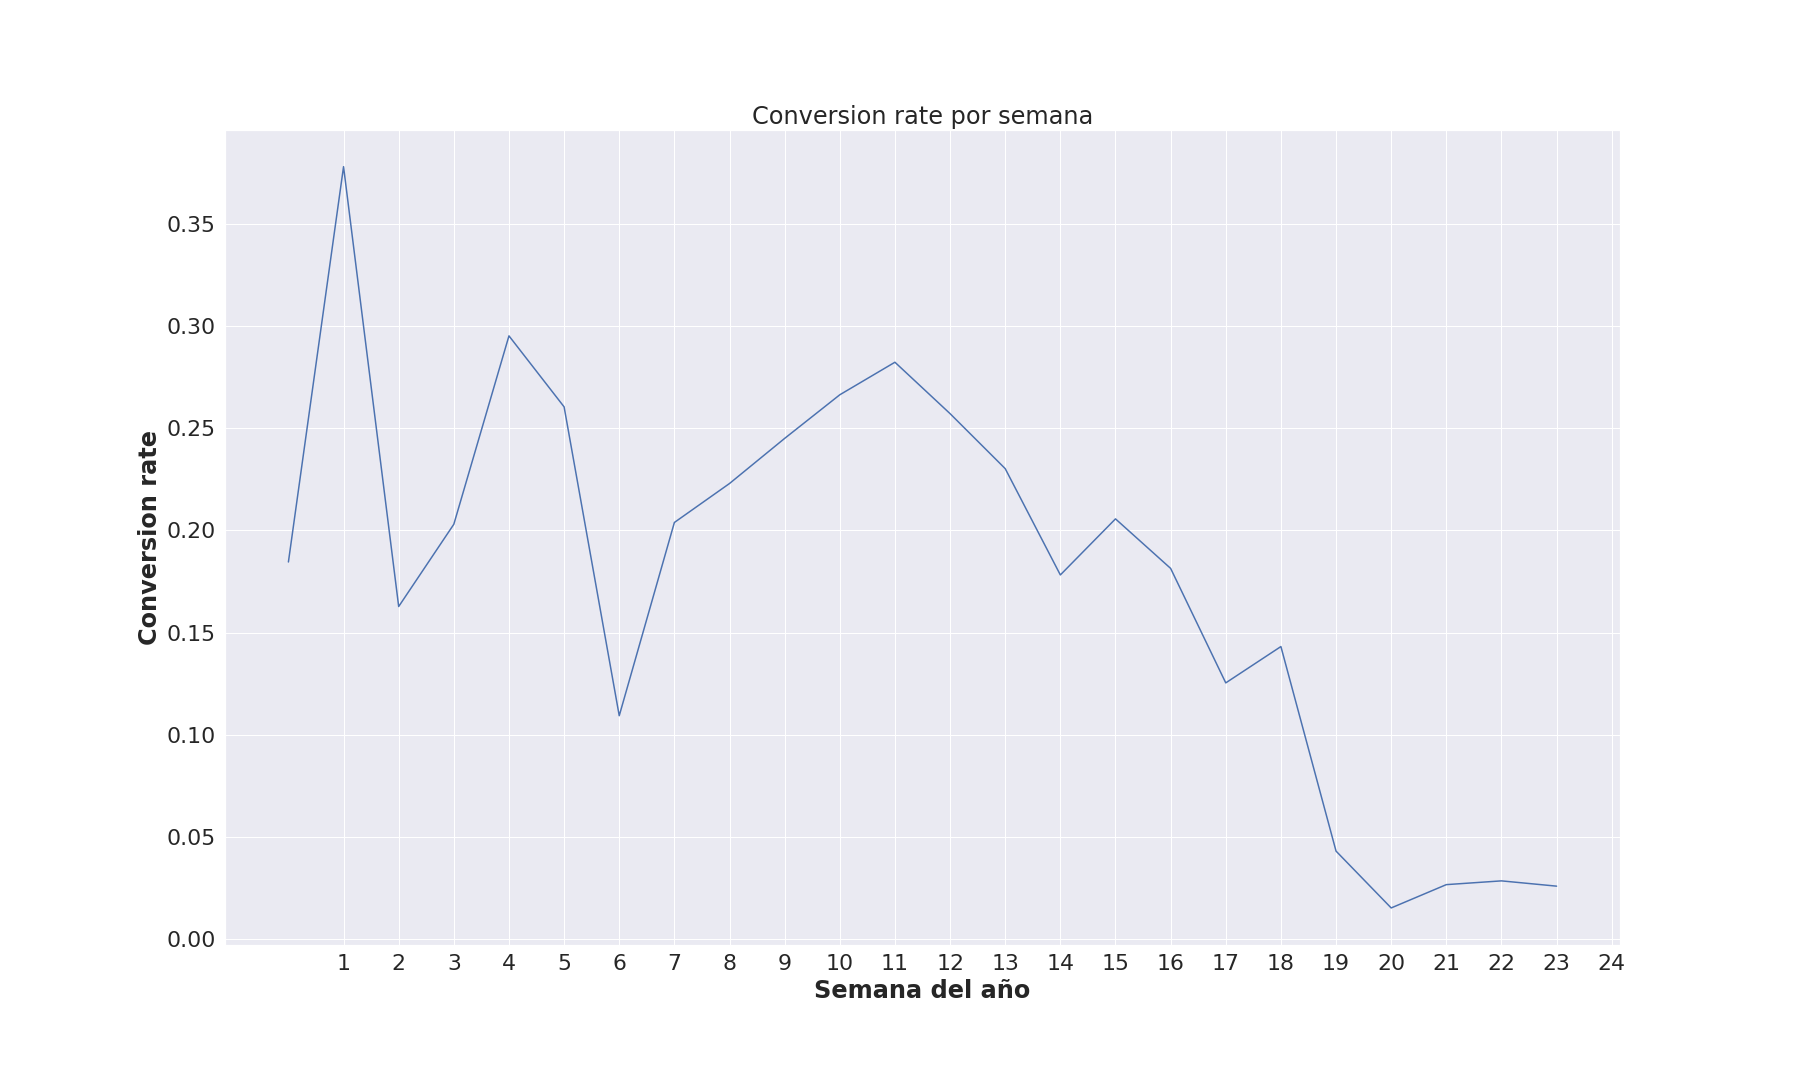
\includegraphics[width=\textwidth]{figures/010-conversion_rate_semana-lineplot.png}
	\caption{Tasa de conversión a lo largo de las semanas del año}
	\label{fig:conversionrate}
\end{figure}

Las mayores tasas de conversiones se registran en las semanas 1,4 y 11, es decir, enero y marzo. Para observar mejor este fenómeno se realiza otro gráfico que muestre la evolución de la tasa de conversión a lo largo de los meses. 

Se refuerza la teoría de que enero y marzo fueron los meses de mayor tasa de conversión. Así mismo, dicha tasa se mantiene estable por 4 meses para luego tener una baja en los meses de mayo y junio. Más adelante se analizarán estos dos meses en profundidad.

\begin{figure}[h!]
	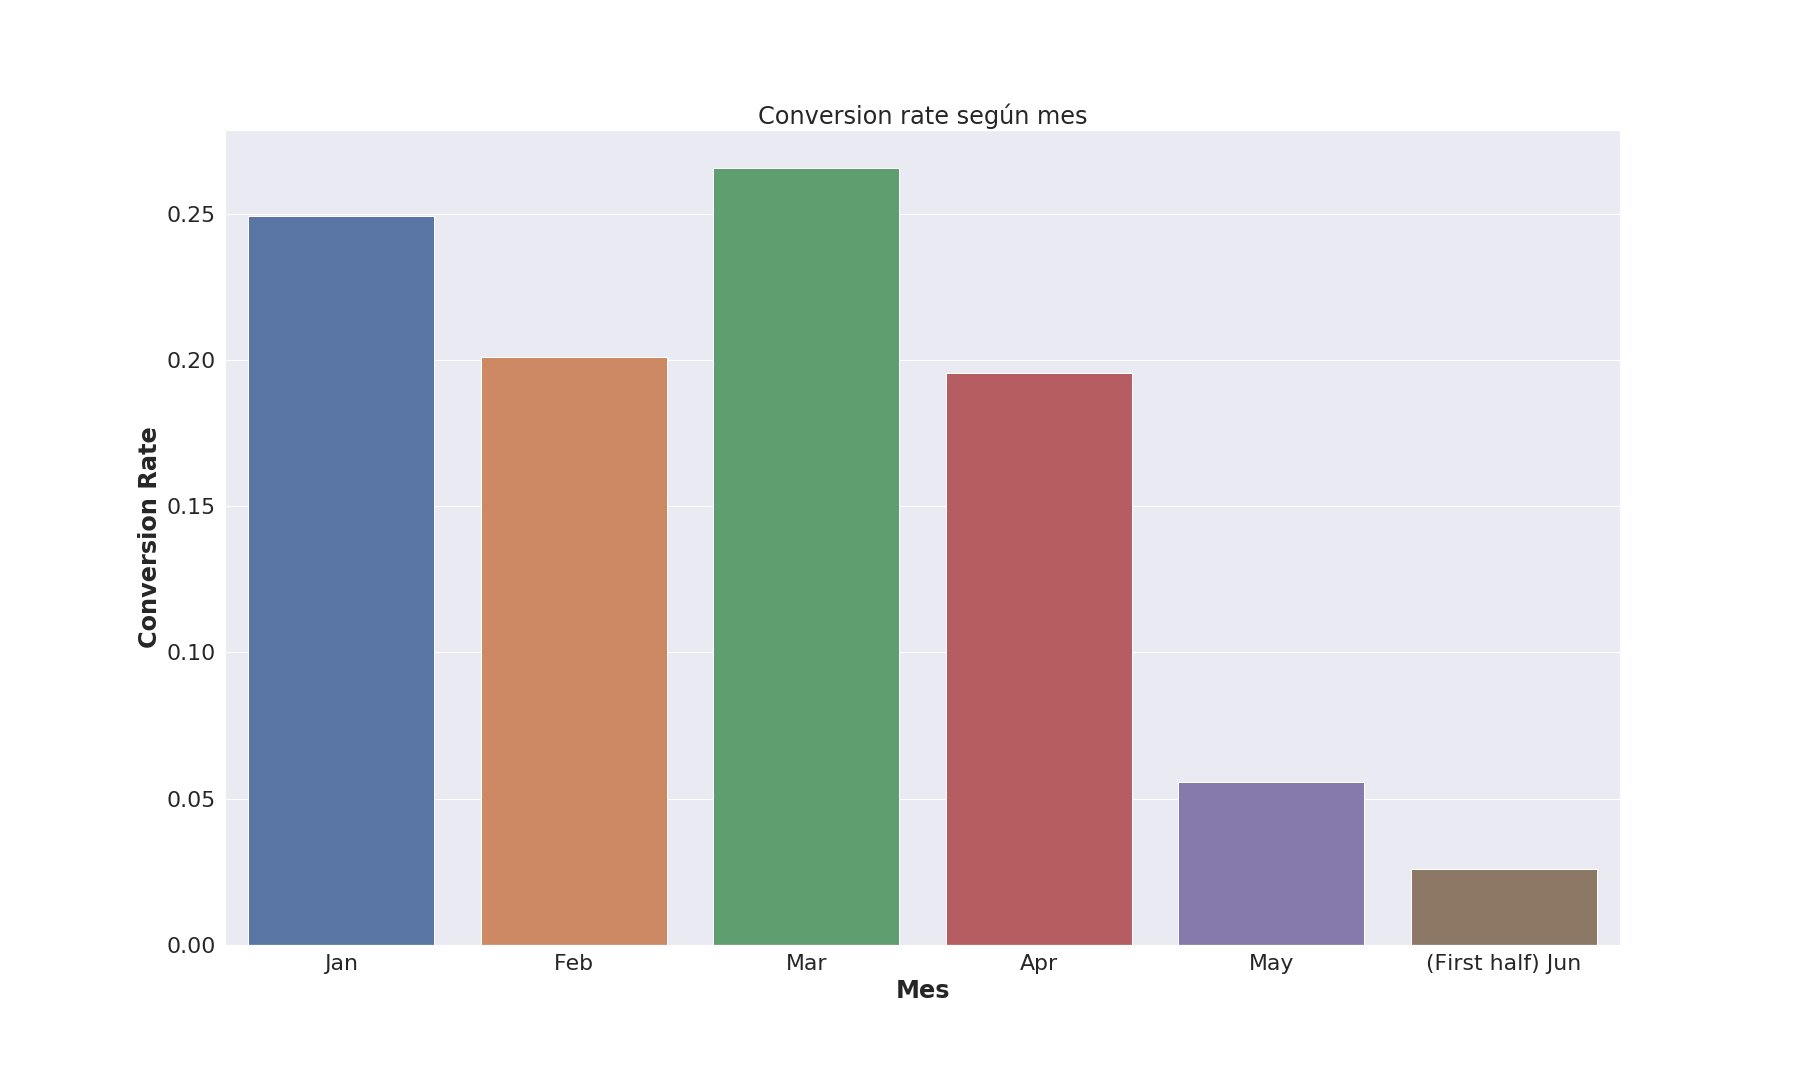
\includegraphics[width=\textwidth]{figures/011-conversion_rate_mes-barplot.png}
	\caption{Tasa de conversión a lo largo de los meses del año}
	\label{fig:conversionratemonthly}
\end{figure}

\subsection{Frecuencia de eventos}

Se analiza qué tipo de evento es el más frecuente en el dataset. Para ello se grafica la cantidad registrada de eventos en función de los distintos tipos de eventos. Se excluyen del análisis los eventos \texttt{checkout} y \texttt{conversion} ya que serán analizados en detalle a lo largo del informe y los eventos \texttt{lead} y \texttt{static page} ya que no se consideran relevantes al análisis que se quiere realizar.

\begin{figure}[h!]
	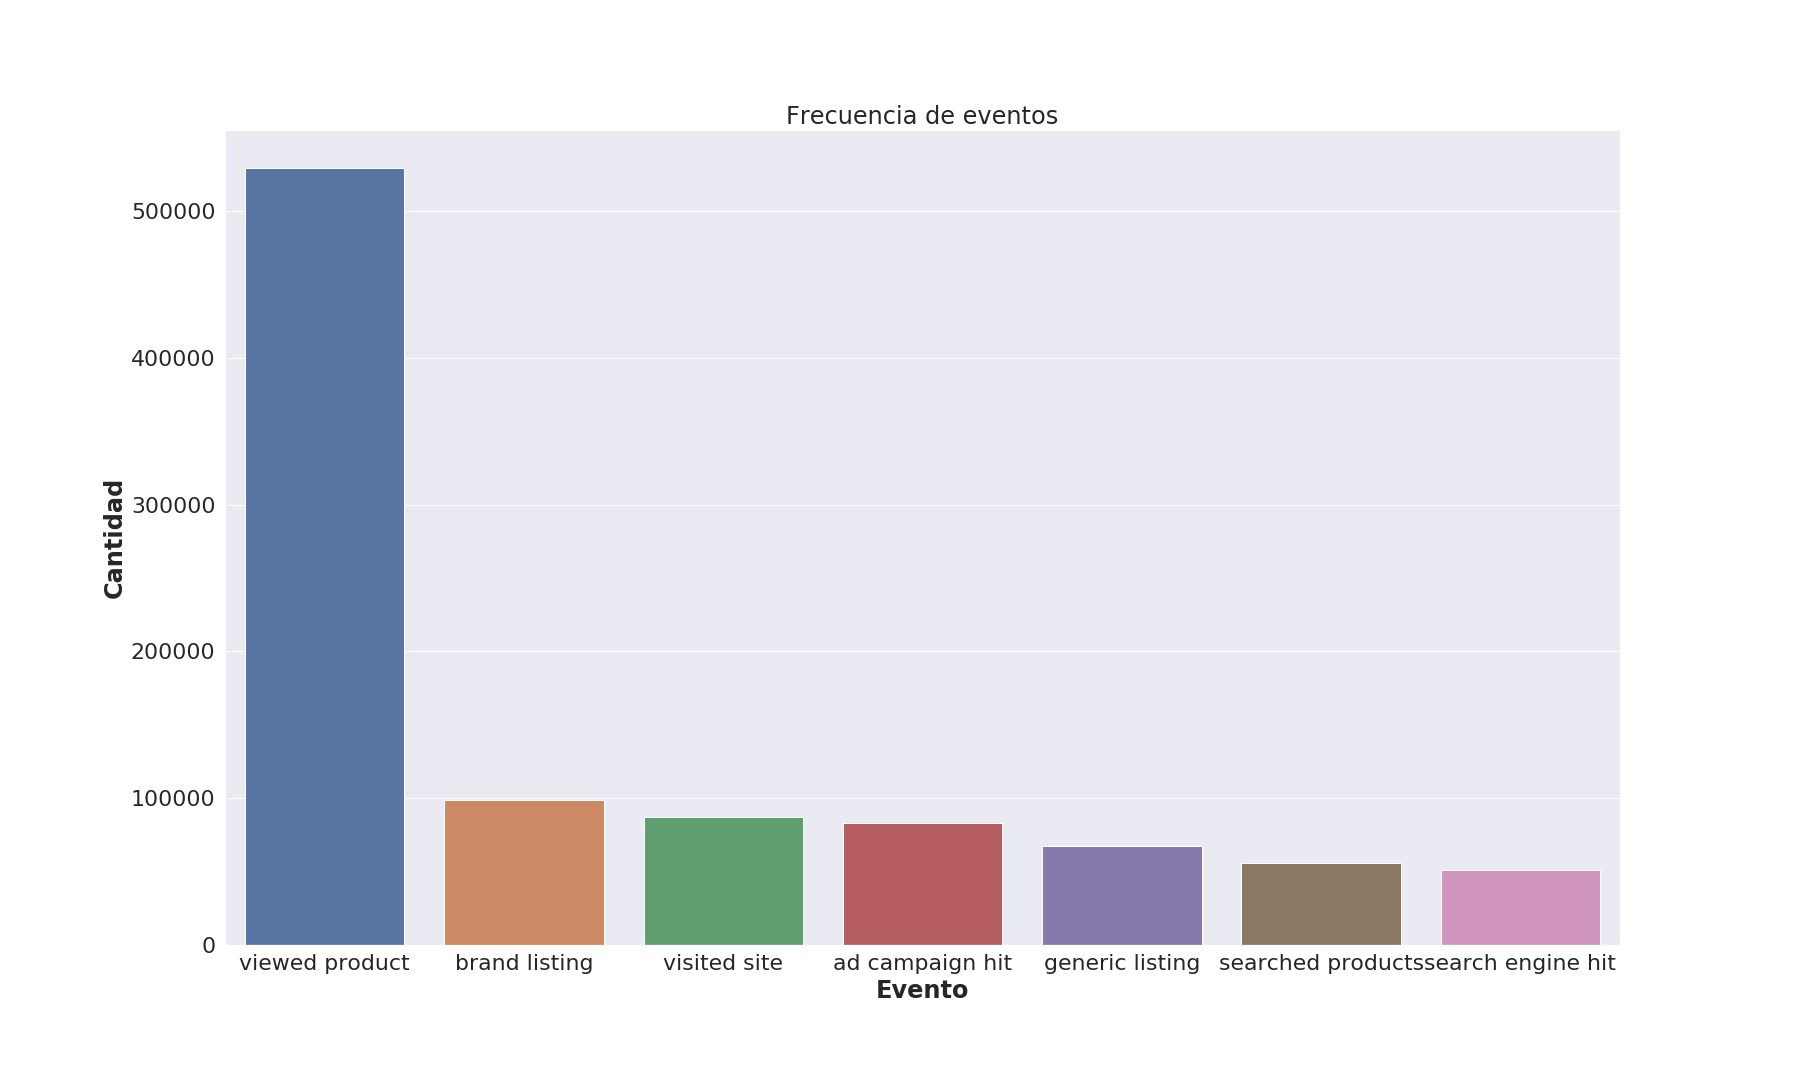
\includegraphics[width=\textwidth]{figures/02-eventos-barplot.png}
	\caption{Frecuencia de eventos}
	\label{fig:freqeventos}
\end{figure}

Se observa en el gráfico que la mayor cantidad de eventos se relacionan a la vista de un producto, lo cual era previsible ya que Trocafone es una plataforma de e-commerce y ver productos constituye su principal función como sitio.

\subsection{Evolución de los eventos a través del tiempo}

\subsubsection{Tráfico del sitio de acuerdo al mes y al día}

Otro aspecto a analizar es la cantidad de eventos producidos en cada día de la semana y del mes. Se busca detectar si se mantiene algún comportamiento específico a lo largo de los meses o si la cantidad de eventos registrada depende de algún factor temporal.

Para realizar este gráfico los datos fueron normalizados para evitar llegar a la conclusión que el mes con una mayor cantidad de eventos es el mes con más eventos por día. 

Se desprende del gráfico que la cantidad de eventos registrada no presenta ningún comportamiento específico. Se observa que dicha cantidad aumenta en la segunda quincena de cada mes pero se considera que la diferencia con el resto de los días no tiene la magnitud suficiente como para extraer alguna conclusión fundada. 

\begin{figure}[h!]
	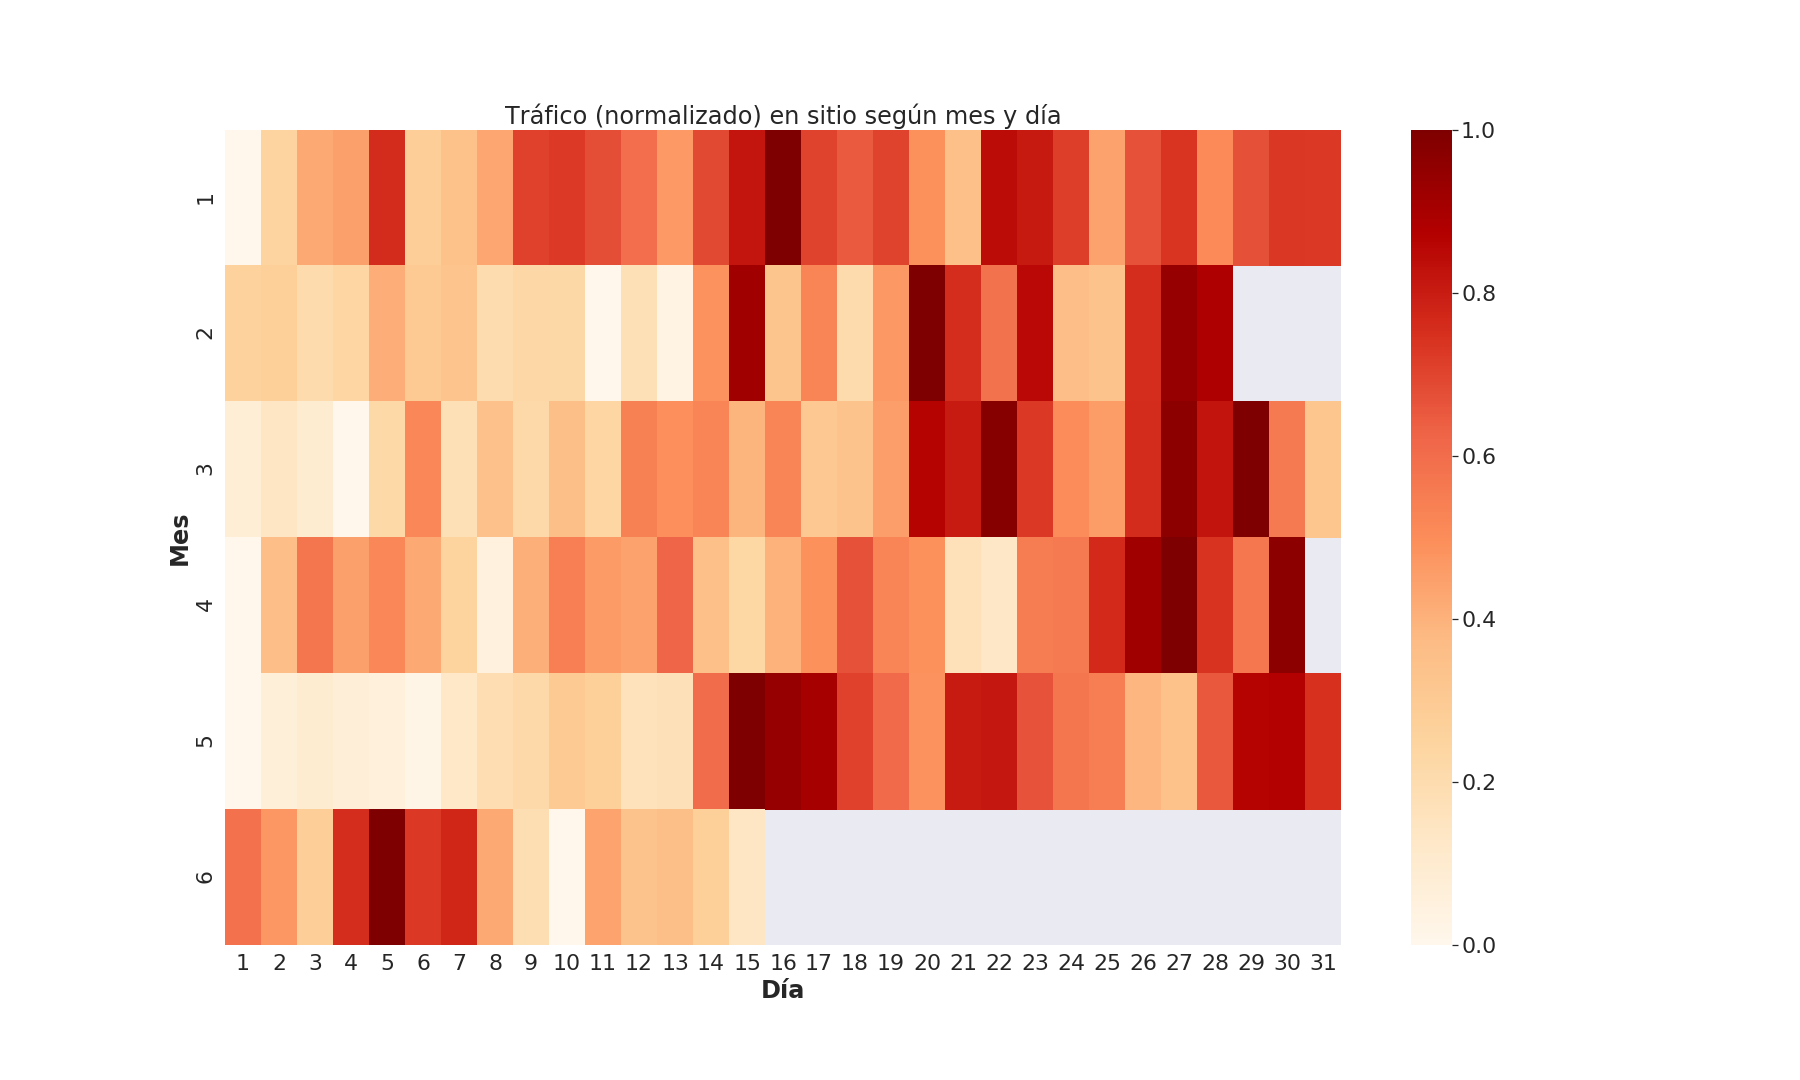
\includegraphics[width=\linewidth]{figures/030-eventos_segun_mes-heatmap.png}
	\caption{Eventos segun mes y día}
	\label{fig:mesdiasnormalizado}
\end{figure}

\subsubsection{Tráfico del sitio de acuerdo al mes y al día de la semana}

En este apartado se busca analizar si algún día de la semana se registra una mayor cantidad de eventos. 

Se realiza un gráfico del mismo estilo que el anterior y se normaliza por las mismas razones.


\begin{figure}[h!]
	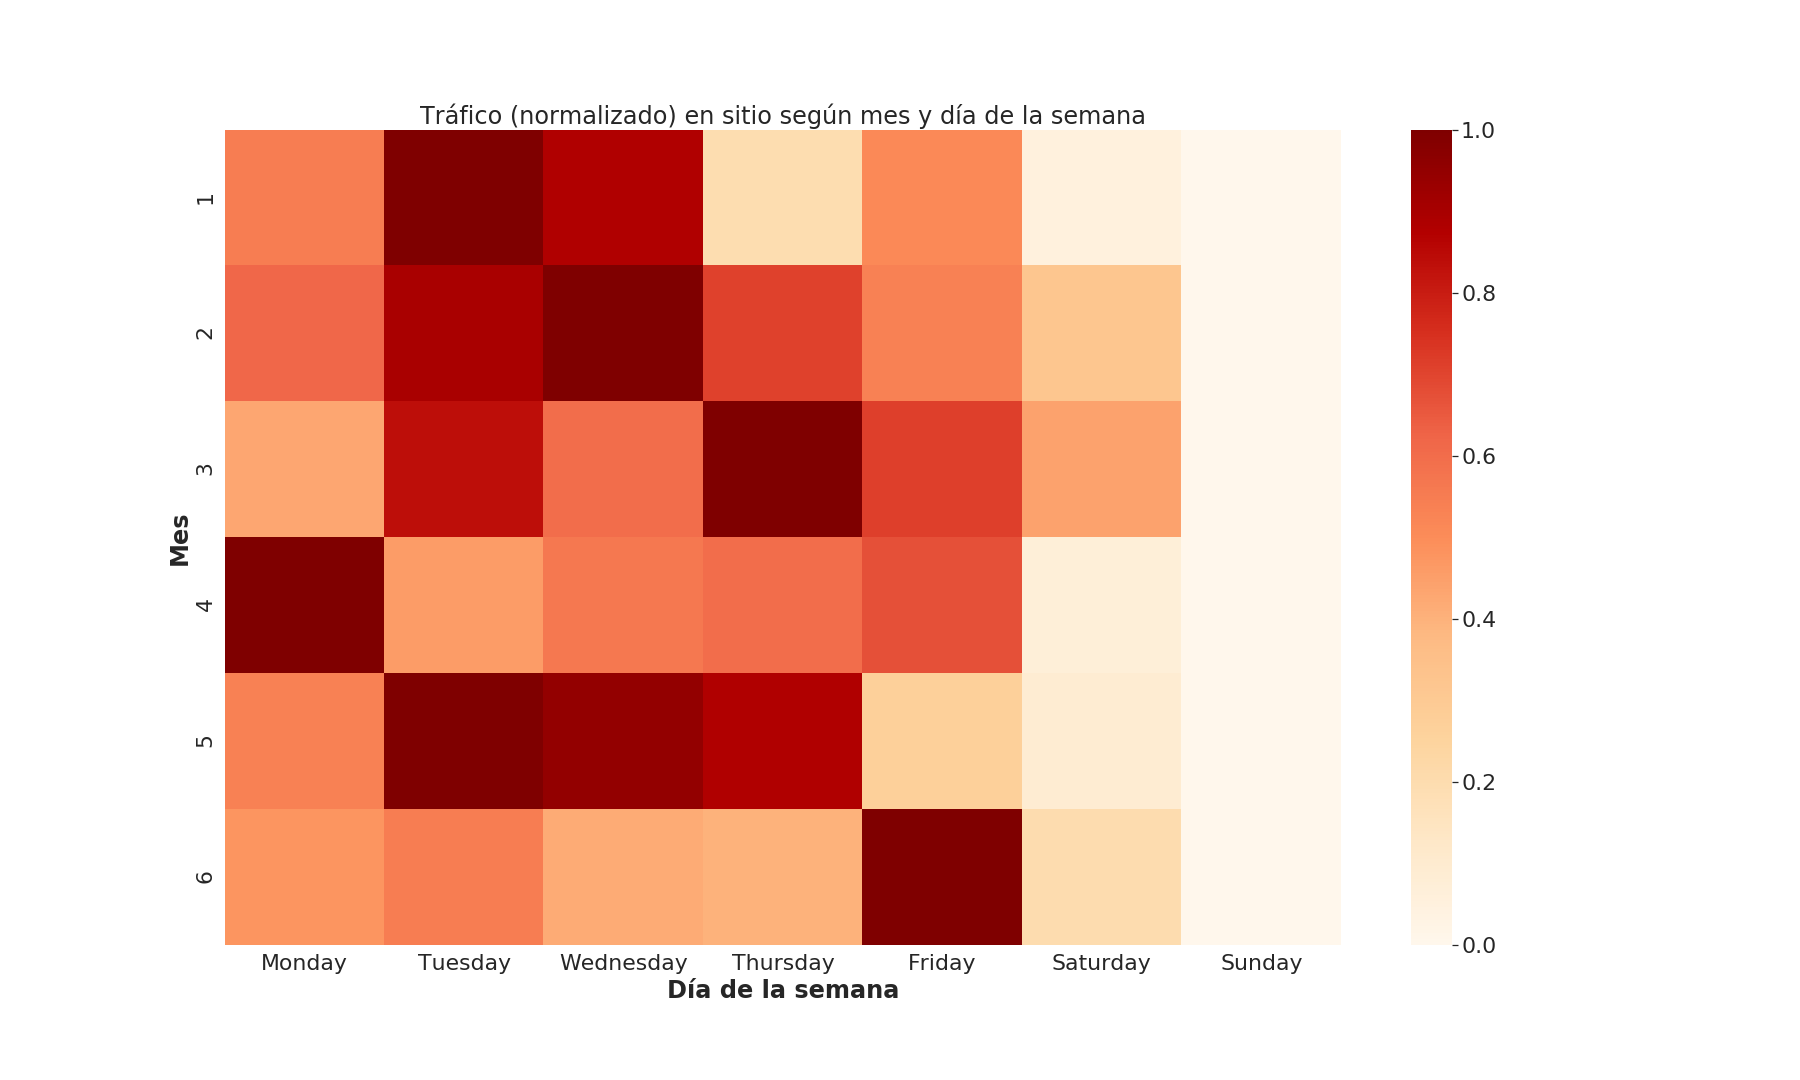
\includegraphics[width=\linewidth]{figures/031-eventos_segun_dow-heatmap.png}
	\caption{Eventos segun mes y día}
	\label{fig:messemanasnormalizado}
\end{figure}

Es notable que durante los días hábiles de la semana el tráfico es mucho mayor que al fin de semana. Esto puede deberse a que los fines de semana suelen ser días de descanso, donde la gente puede no estar pensando en realizar una compra, además de no poder retirarla. En la semana aumenta el tráfico debido a que el envío o el retiro del celular puede realizarse en el momento.

\subsubsection{Tráfico del sitio según mes}

En este apartado se busca analizar si en algún mes se registró una mayor cantidad de eventos o si la distribución de las visitas fue uniforme a lo largo del tiempo.

\begin{figure}[h!]
	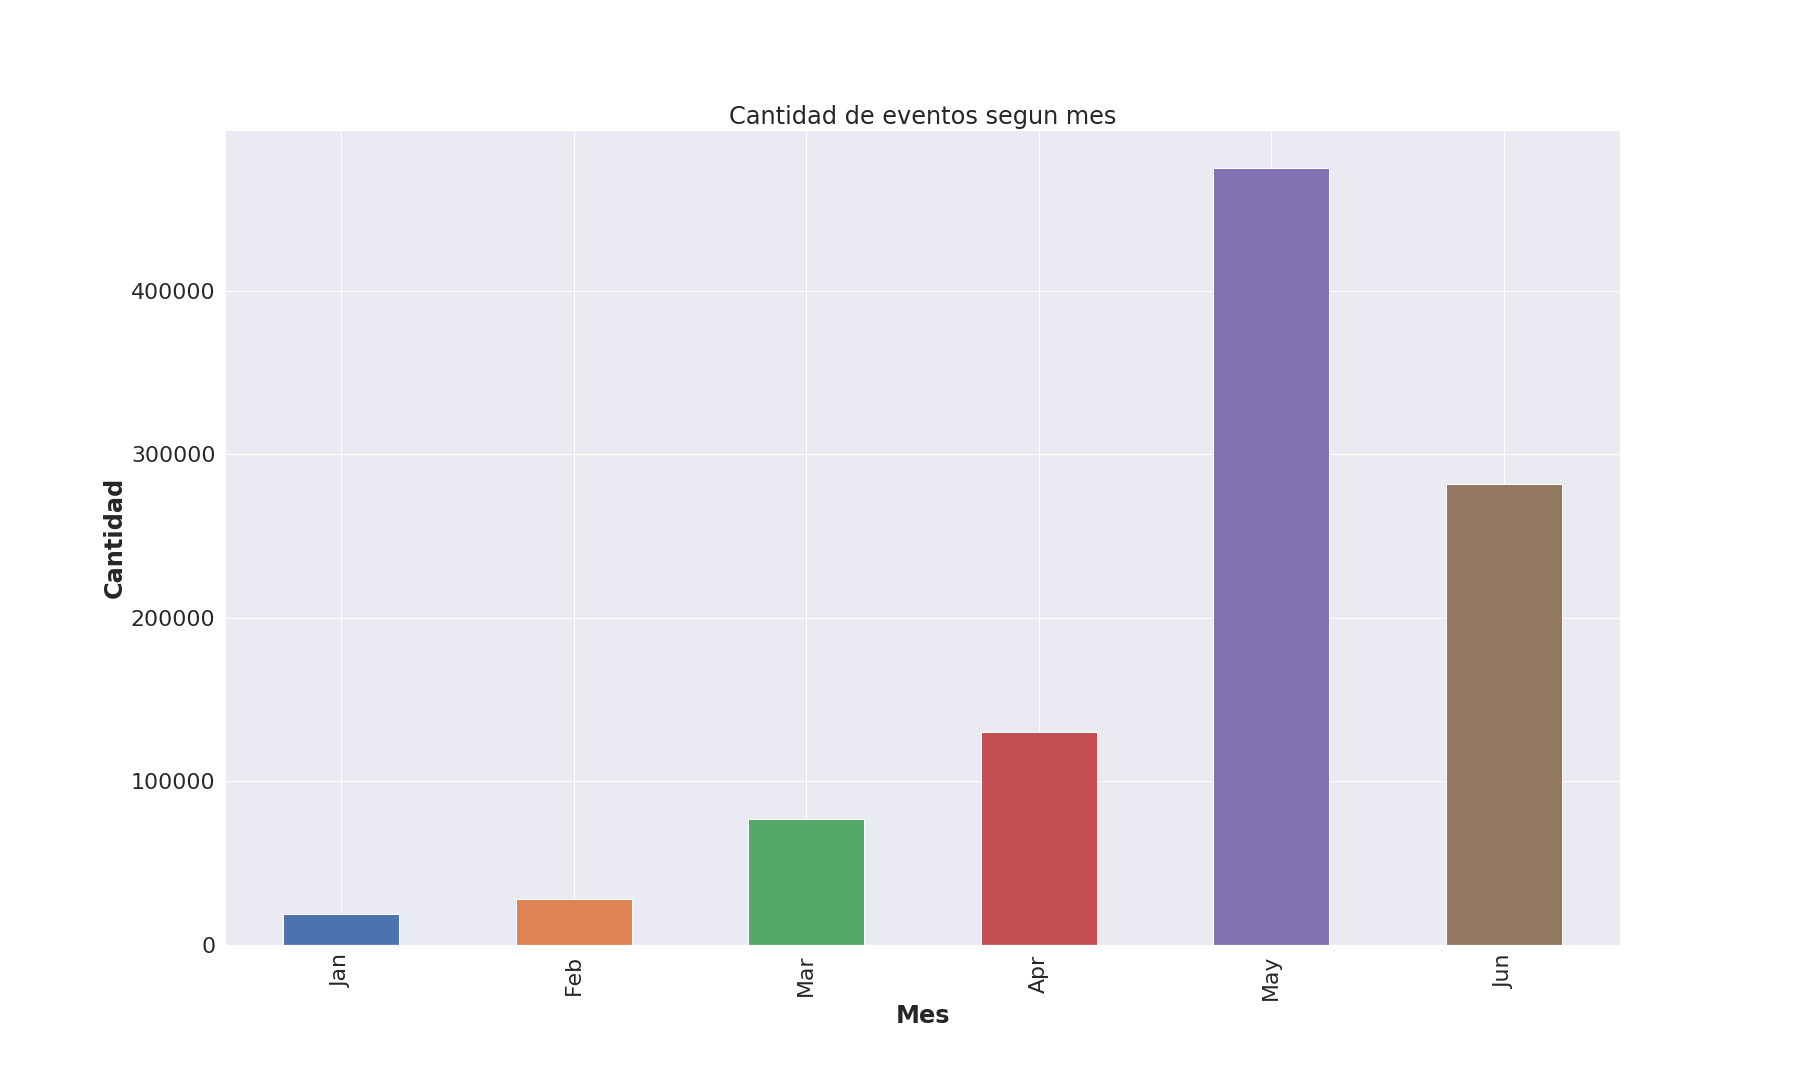
\includegraphics[width=\linewidth]{figures/032-eventos_segun_mes-barplot.png}
	\caption{Eventos segun mes}
	\label{fig:mes}
\end{figure}

Los meses de mayo y junio registraron una cantidad notablemente mayor de eventos. Este resultado llama la antención por lo que se analiza en mayor profundidad en la próxima sección. Es importante destacar que esta evolución es inversa a la de la tasa de conversión. Se concluye que en mayo si bien no hubo tantas ventas, sí aumentó mucho la cantidad de eventos. 

\subsubsection{¿Por qué mayo y junio registran una mayor cantidad de eventos?}

Para tratar de encontrar una respuesta a esta pregunta se centraliza el análisis en estos meses y se estudian los tres eventos principales del dataset: \texttt{conversion}, \texttt{checkout} y \texttt{viewed products}.

\begin{figure}[h!]
	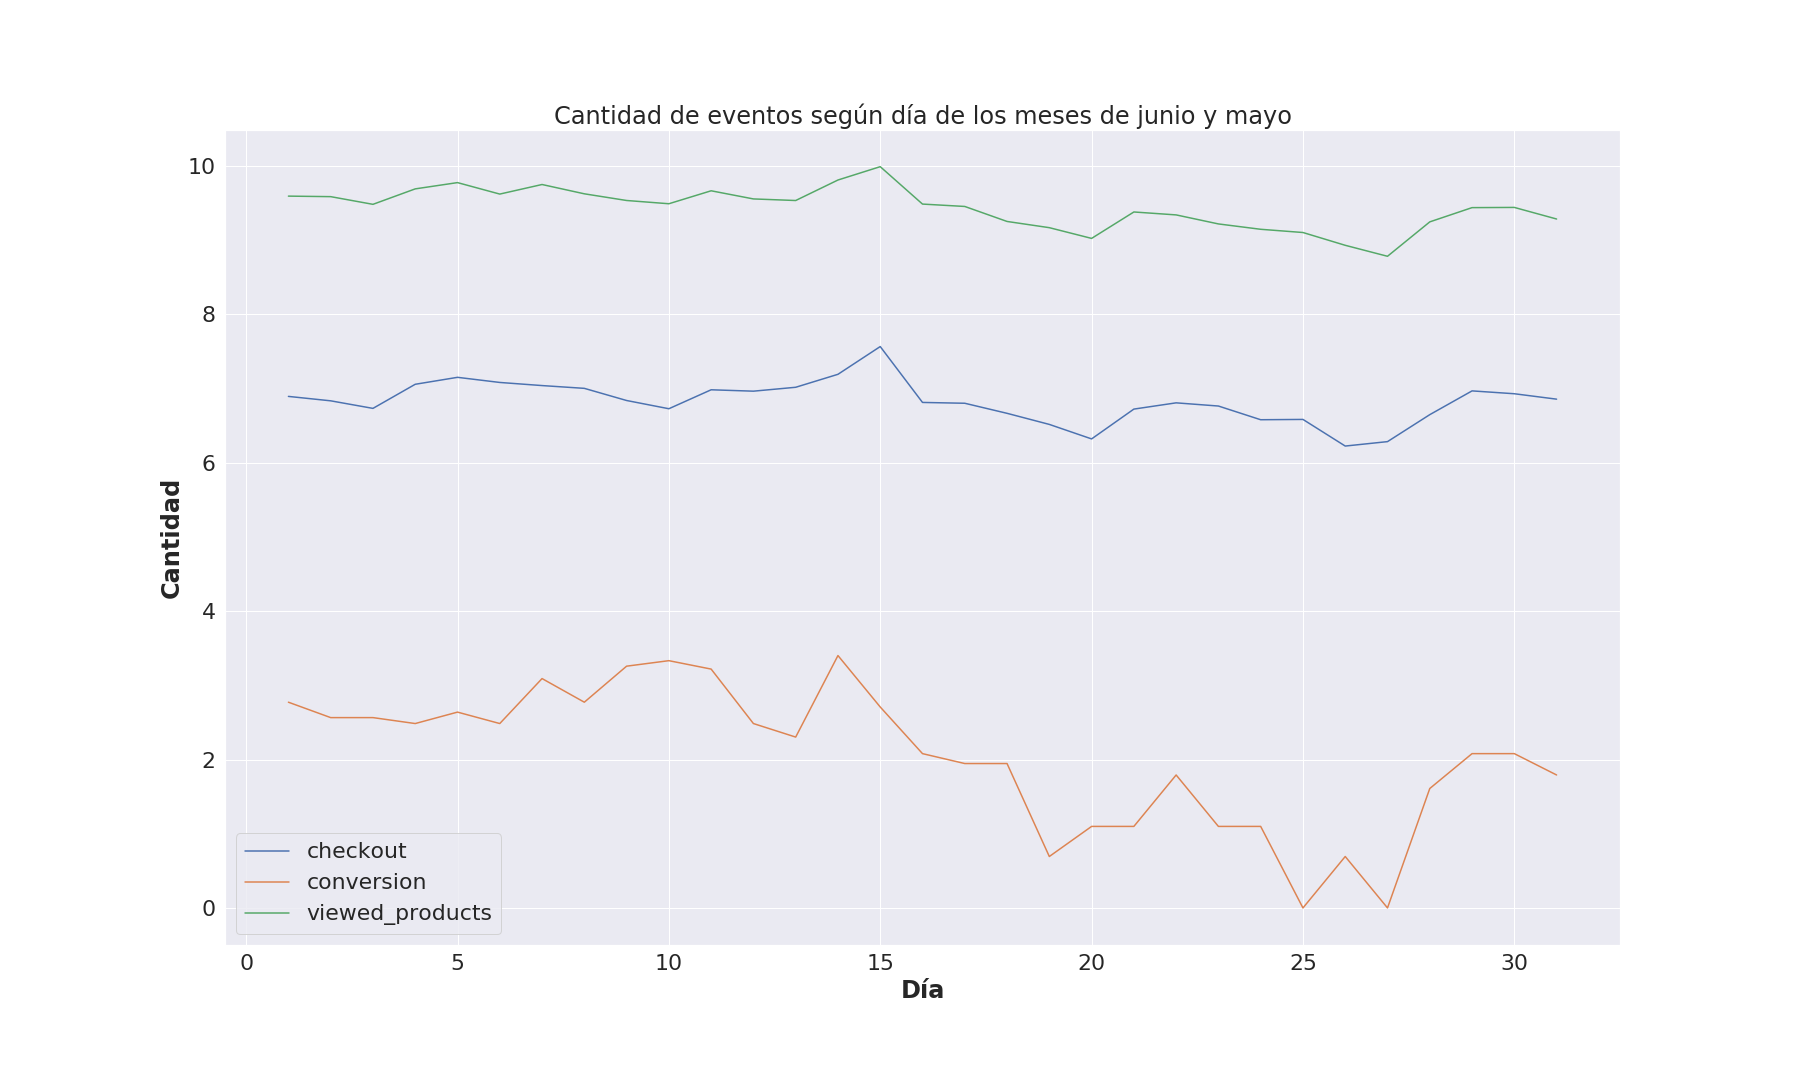
\includegraphics[width=\linewidth]{figures/033-eventos_mayo_junio_lineplot.png}
	\caption{Conversiones, checkouts y viewed products a lo largo de los días del mes de mayo y junio en éscala logarítmica}
	\label{mayojunio}
\end{figure}

Los tres eventos presentan su máximo alrededor de los días 14 a 16. Como Trocafone es del país de Brasil y el mayor tráfico proviene de allí, lo cual será verificado posteriormente, se infiere que puede deberse a alguna promoción lanzada en la plataforma o en el mismo país. Esto no puede concluirse con certeza debido a la falta de información en internet y en la plataforma de promociones pasadas.

\subsubsection{Hora de mayor cantidad de conversiones y checkouts}

En un intento de encontrar un comportamiento patrón por parte de los clientes se grafica la cantidad de conversiones y de checkouts en función de las horas del día. Se busca determinar la hora en la que ambas confluyan en su máximo para analizar el motivo por el que dicha hora registra mayor tráfico.

Se observa que ambos gráficos confluyen en su máximo a las 19 hs. Esto puede significar que la mayoría de los usuarios cuando vuelven del trabajo o están finalizando su día deciden realizar conversiones o checkouts. La diferencia entre ambos gráficos es que la cantidad de checkouts realizados se mantiene relativamente constante en las segundas 12 hs del día mientras que las conversiones son mucho menores y presentan picos más marcados en los horarios de la tarde-noche. 

\begin{figure}[h!]
	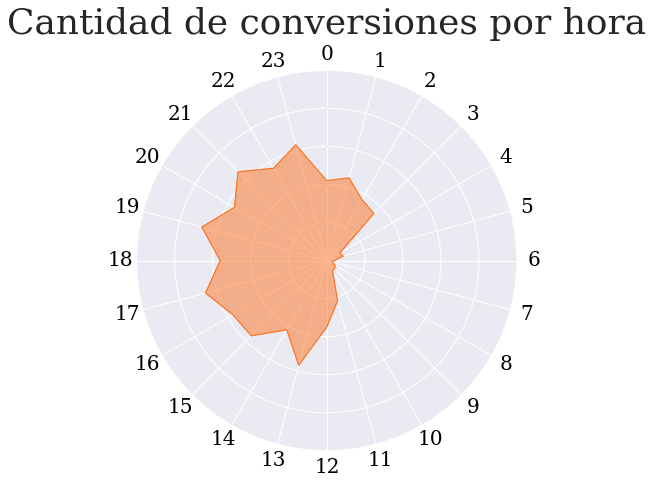
\includegraphics[width=6cm,height=6cm,keepaspectratio]{figures/040-hours-conversion-radarchart.png}
	\caption{Conversiones a lo largo de las horas del día}
	\label{conversionclock}
\end{figure}

\begin{figure}[h!]
	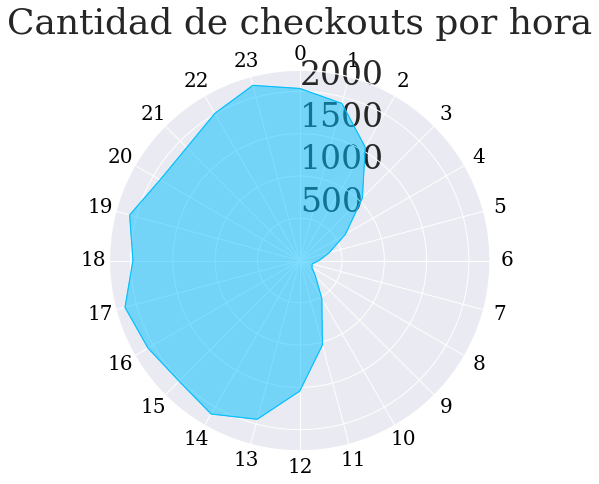
\includegraphics[width=6cm,height=6cm,keepaspectratio]{figures/041-hours-checkout-radarchart.png}
	\caption{Checkouts a lo largo de las horas del día}
	\label{checkoutclock}
\end{figure}

\section{Análisis geográfico}

En este apartado se busca analizar las ciudades, países y regiones de dónde provienen los distintos tipos de eventos. Trocafone es una empresa que inició en Brasil y expandió sus comercios a Argentina en el 2015, por lo que se deduce que probablemente Brasil sea la zona de mayor influencia en los eventos.

\subsection{Países que registran mayor cantidad de eventos} 

\begin{figure}[h!]
	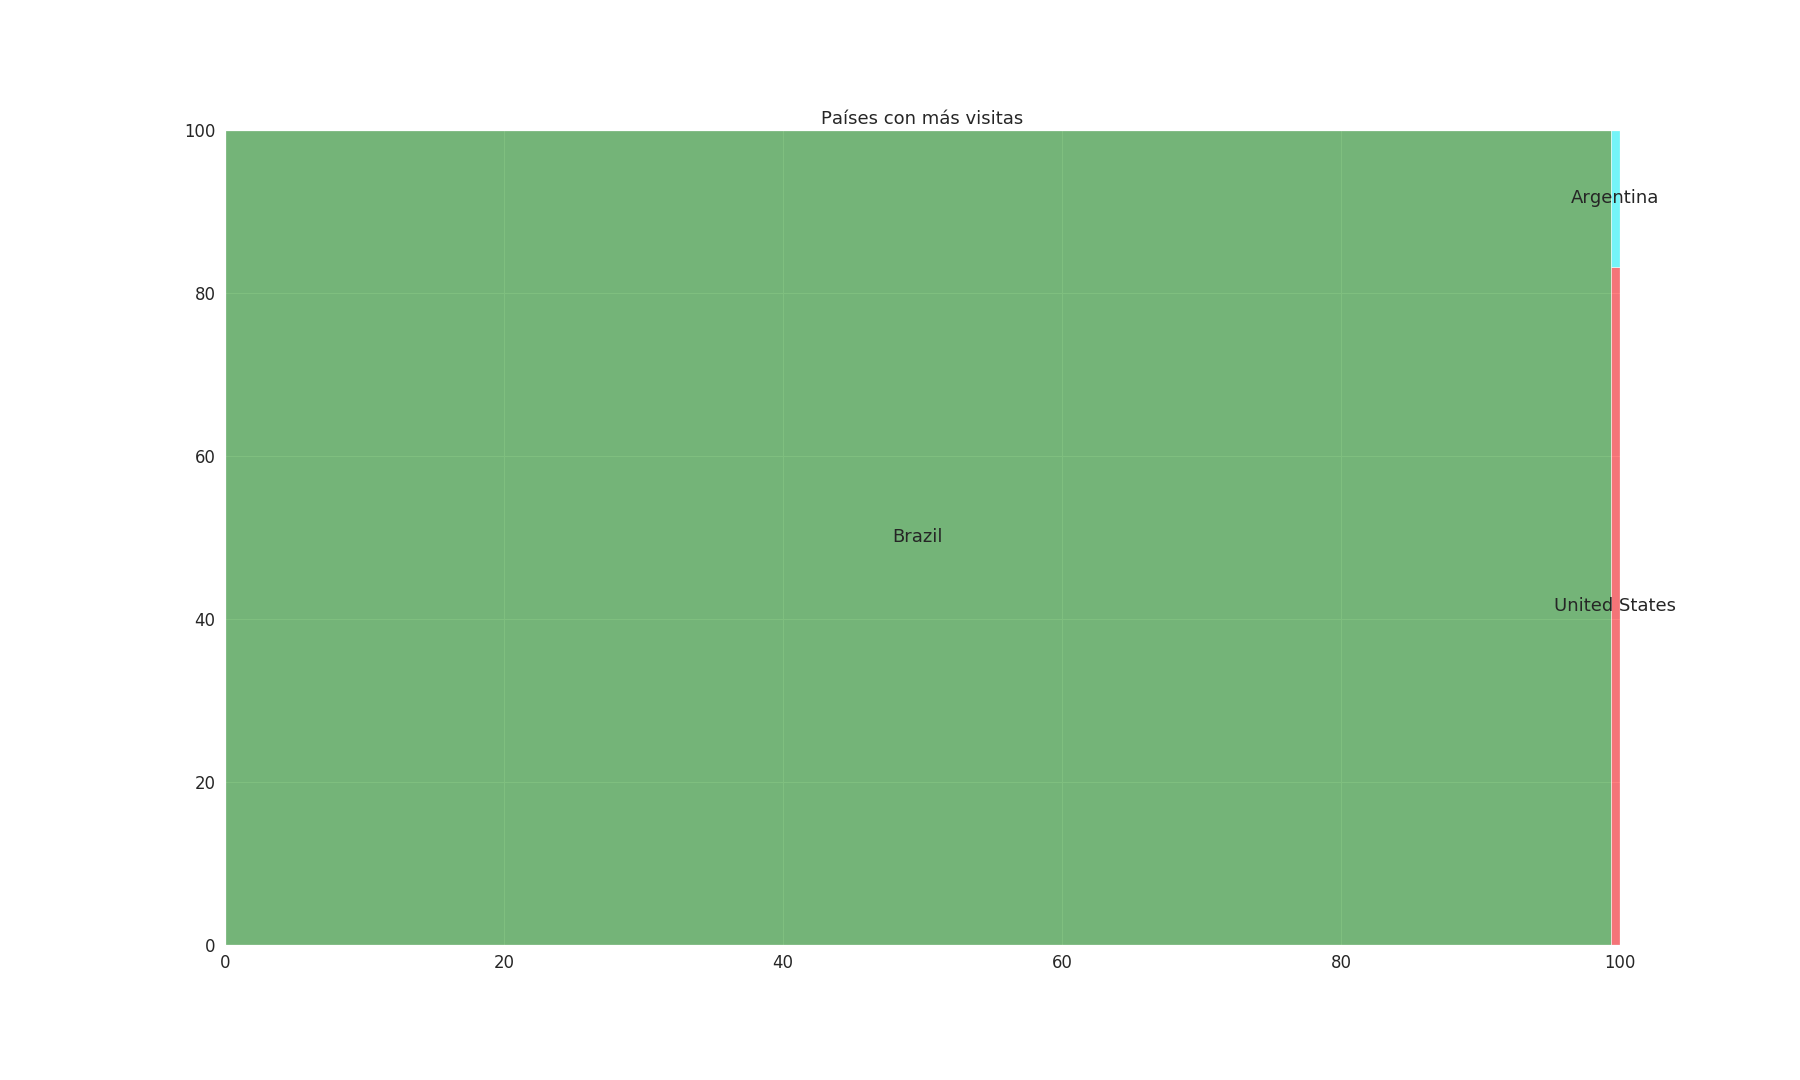
\includegraphics[width=\linewidth]{figures/050-paises_visitas-treemap.png}
	\caption{Países de mayor tráfico de la página}
	\label{brazilrules}
\end{figure}

\begin{figure}[h!]
	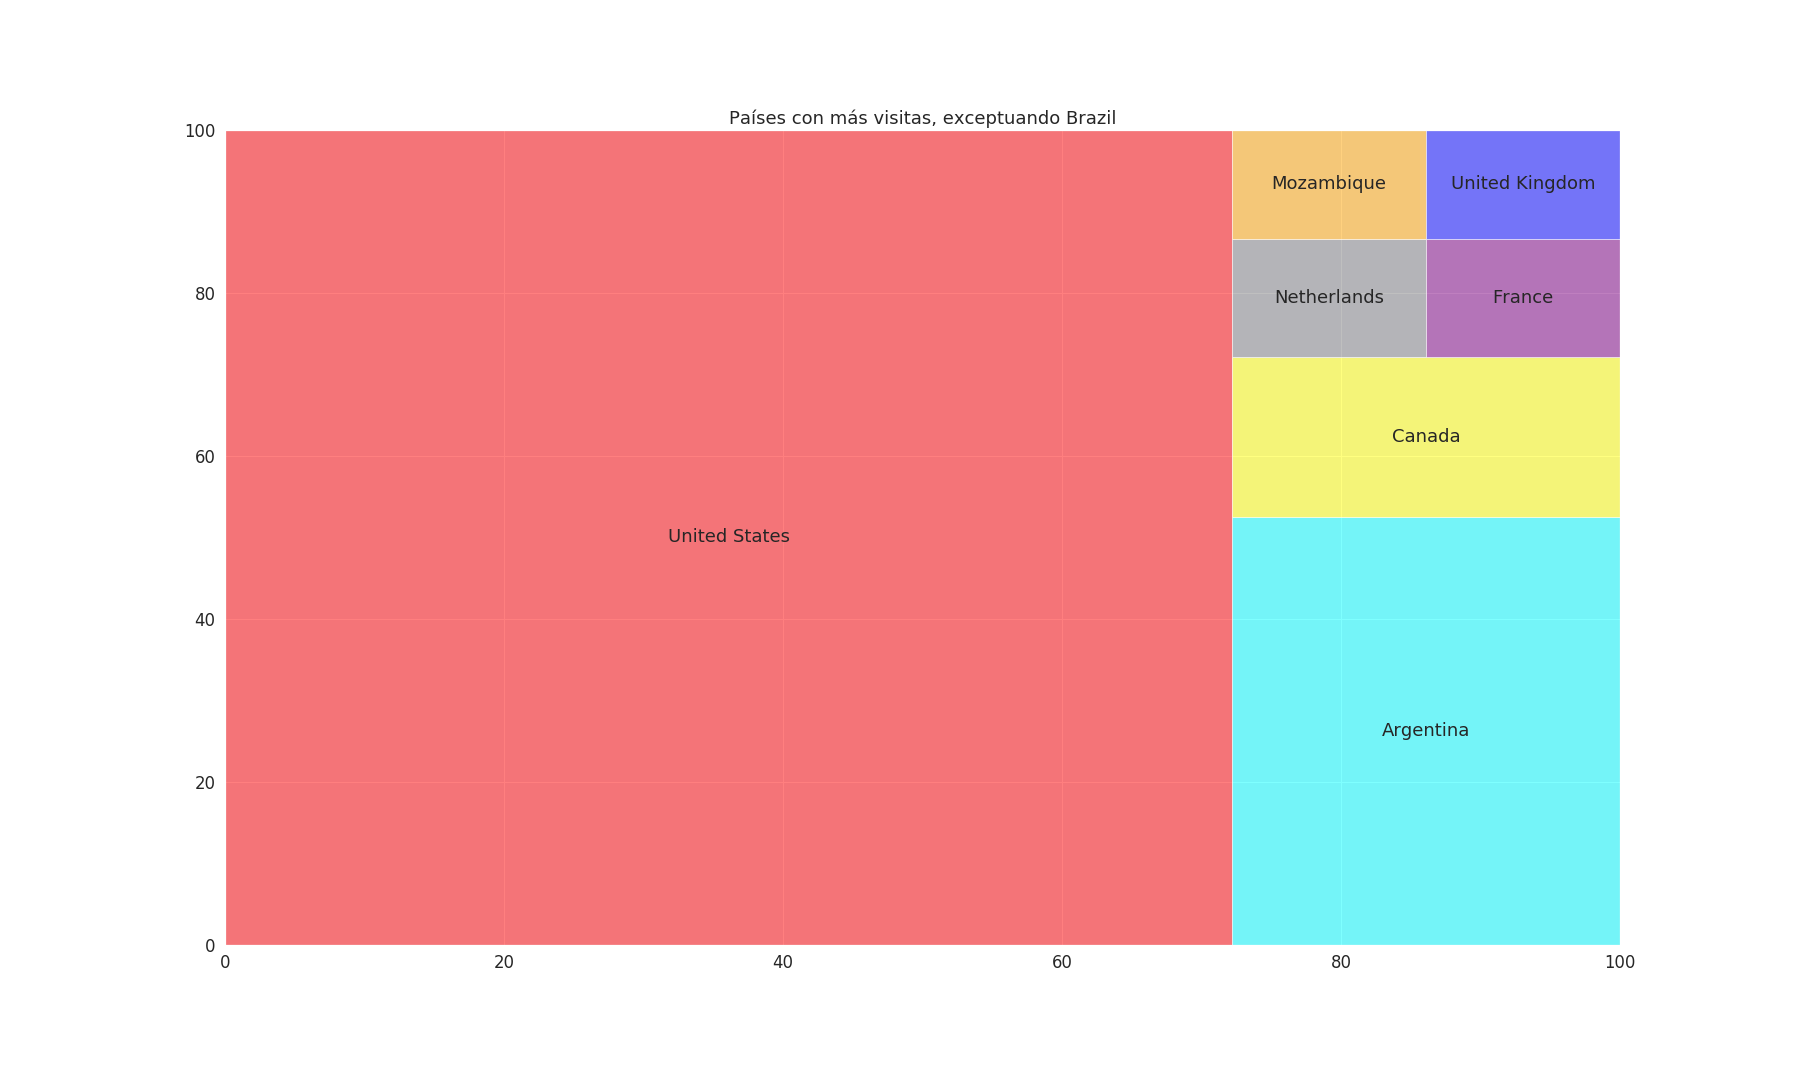
\includegraphics[width=\linewidth]{figures/051-paises_visitas_sin_brazil-treemap.png}
	\caption{Países de mayor tráfico de la página sin contar a Brasil}
	\label{brazilsucks}
\end{figure}

Se corroboró la teoría inicial por lo que se procedió a eliminar a Brasil del gráfico para poder observar qué otros países intervienen en la página de Trocafone. Estados Unidos supera en una amplia cantidad la influencia en la página a Argentina, a pesar de ser una de las sedes de la empresa. Esto puede explicarse debido a que la gran mayoría de los eventos no son conversiones, por lo tanto es mactible que cualquier persona de los Estados Unidos busque celulares en la plataforma, sin llegar a registrar un evento de tipo \texttt{checkout} o \texttt{conversión}.

\subsection{Regiones y ciudades que registran mayor cantidad de eventos}

Se procede a analizar qué ciudades y regiones de Brasil son las que registran mayor cantidad de eventos. Para ello se grafica las regiones con una mayor cantidad de visitas. Se observa que las tres regiones con la mayor cantidad de eventos (San Pablo, Minas Gerais y Rio de Janeiro) están sobre la costa del sudeste. Para visualizar esto de una mejor manera se realiza un gráfico que muestra las ciudades de Brasil más visitadas y se verifica que la mayoría de los eventos se producen sobre la costa sudeste.

\begin{figure}[h!]
	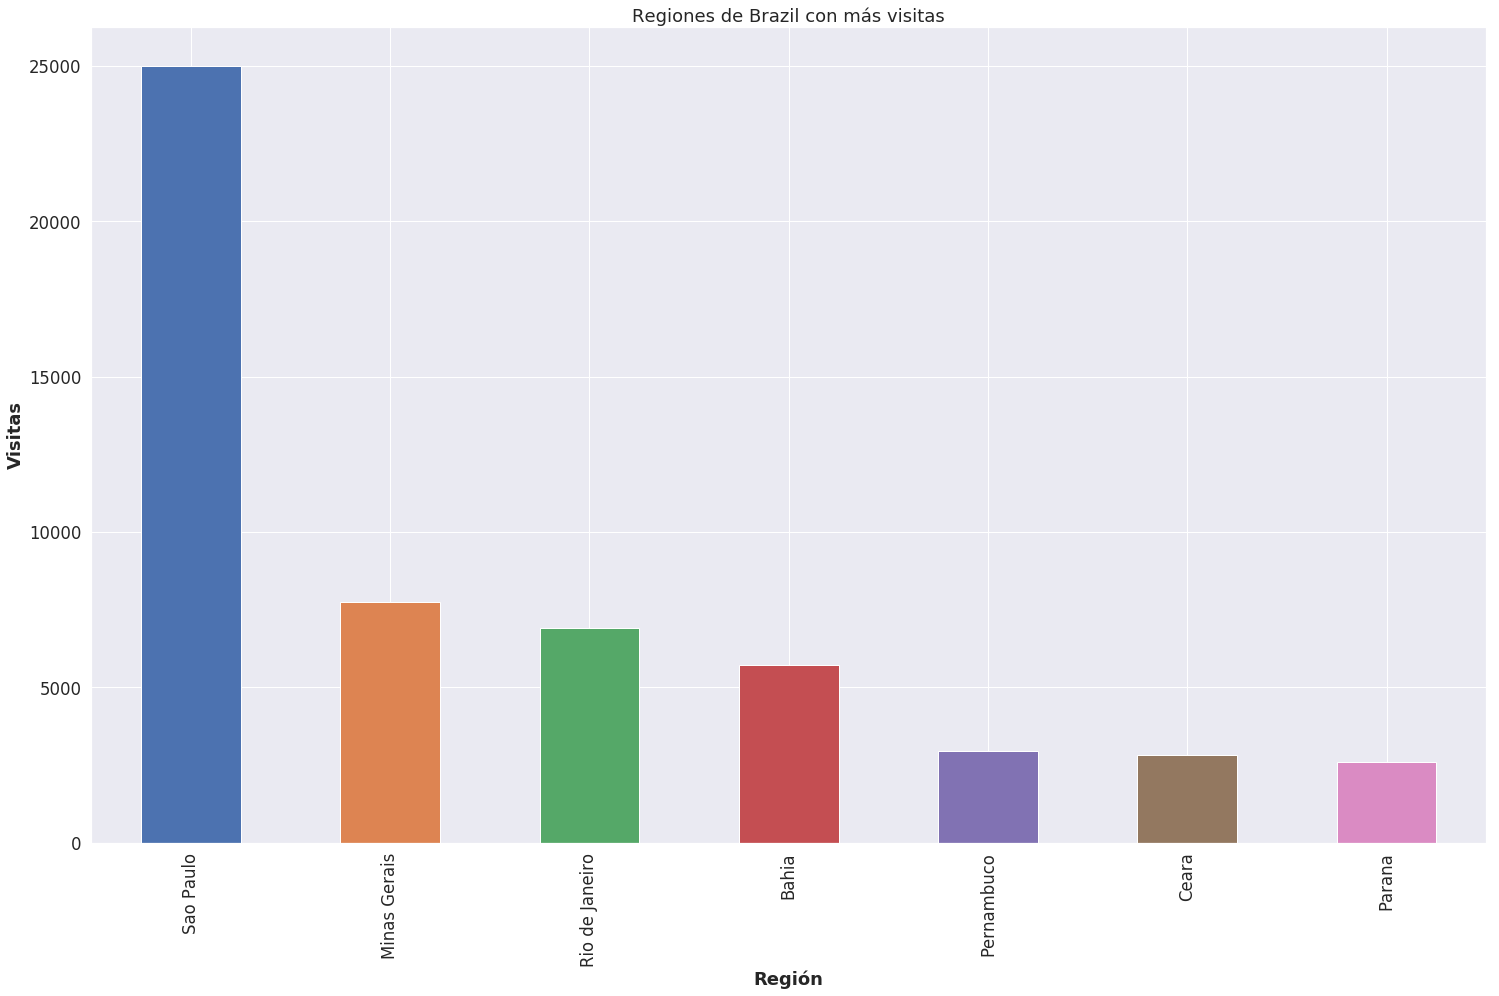
\includegraphics[width=9cm,height=9cm,keepaspectratio]{figures/060-regiones_brazil-barplot.png}
	\caption{Regiones de Brasil con mayor cantidad de eventos}
	\label{regionsbrasil}
\end{figure}

\begin{figure}[h!]
	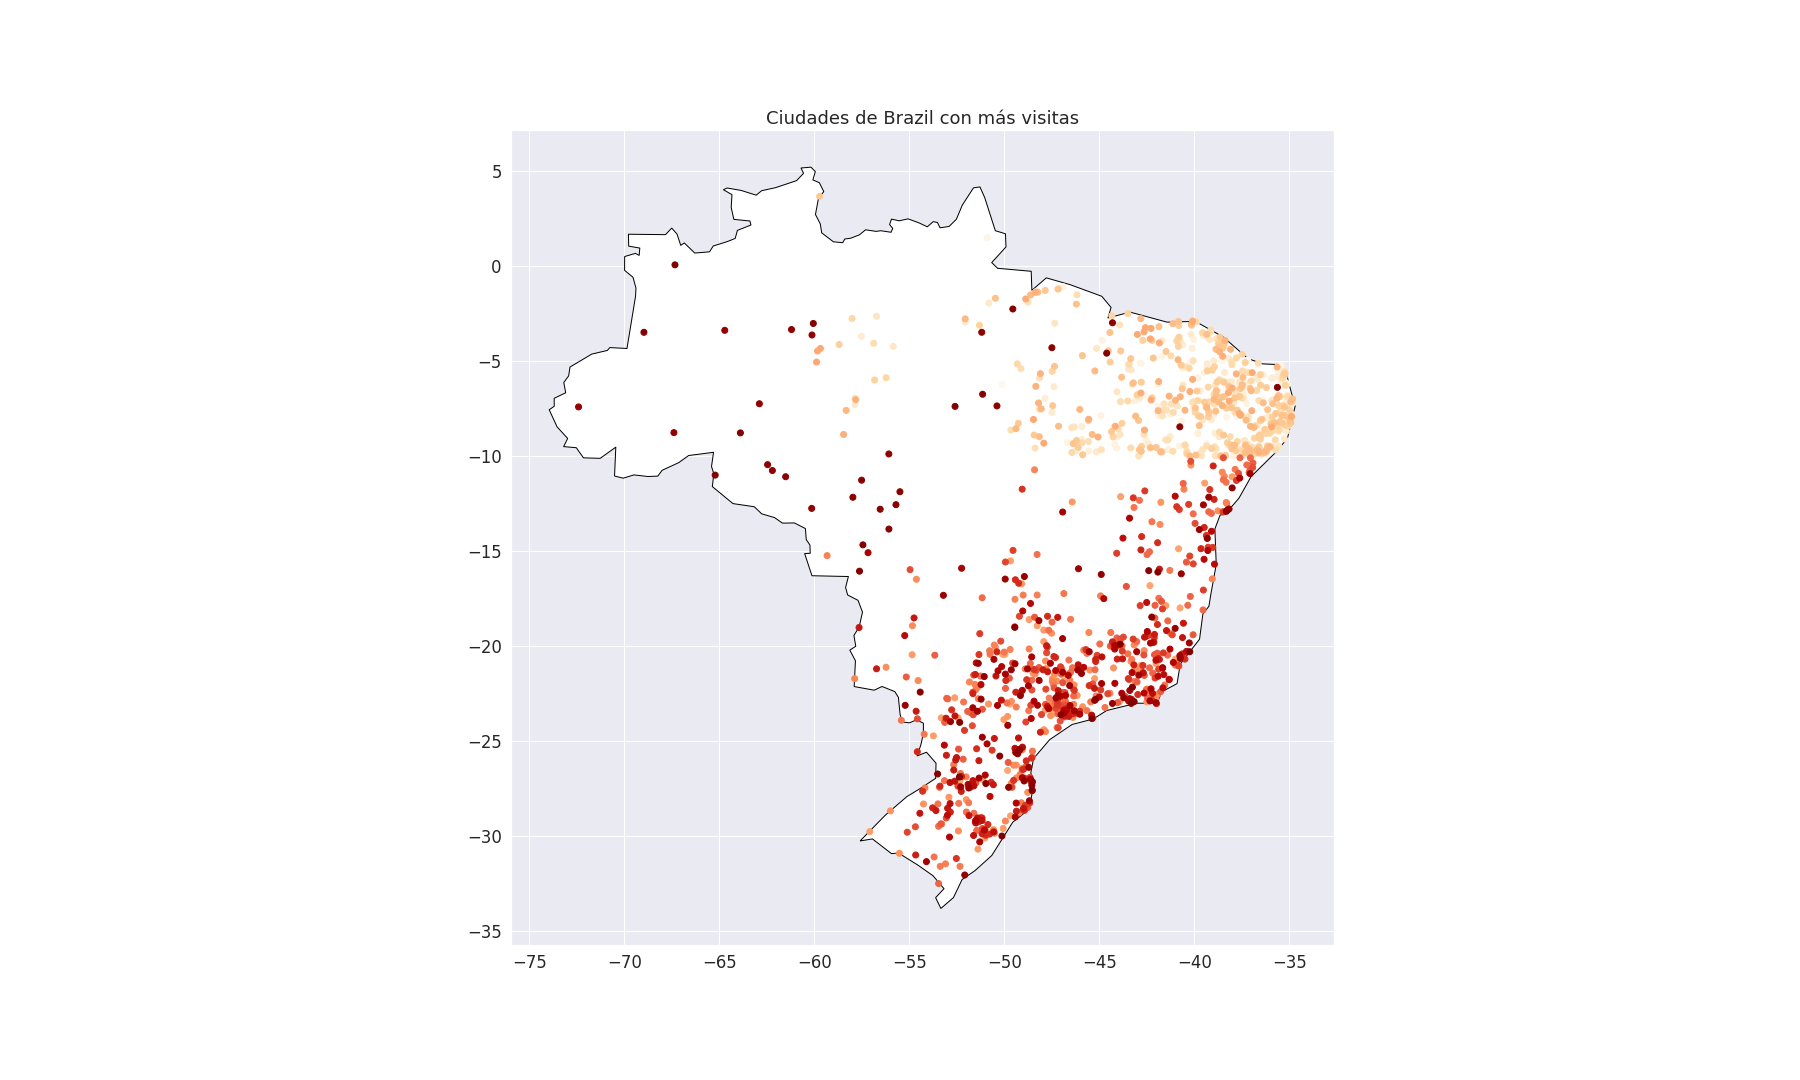
\includegraphics[width=11cm,height=11cm,keepaspectratio]{figures/061-ciudades_brazil-choropleth.png}
	\caption{Ciudades de Brasil con mayor cantidad de eventos}
	\label{citybrasil}
\end{figure}

\section{Análisis de búsquedas}

La idea de este apartado radica en analizar los términos que buscan los usuarios en la plataforma y así identificar ciertos patrones de búsqueda como por ejemplo cuál es el modelo de celular más buscado. Este análisis se dividirá en dos:

\begin{itemize}
	\item \underline{Términos ingresados en el buscador}: se utiliza la columna \texttt{search\_term} del dataframe.
	\item \underline{Productos buscados en la plataforma}: se utiliza la columna \texttt{event} del dataframe para buscar aquellos eventos que correspondan a \texttt{searched\_product}.
 \end{itemize}

\subsection{Términos ingresados en el buscador}

Se realiza un gráfico para visualizar a grandes rasgos los términos más buscados por los usuarios. Se busca tener una idea aproximada de los modelos de celular más requeridos o deseados por los usuarios. Figuran en el gráfico los términos que fueron buscados como mínimo 300 veces, un número arbitrario impuesto para fijar un límite mínimo de búsquedas para ser considerado de los más buscados. De no fijar este límite el gráfico estaría sobrecargado y sería difícil de interpretar.

\begin{figure}[h!]
	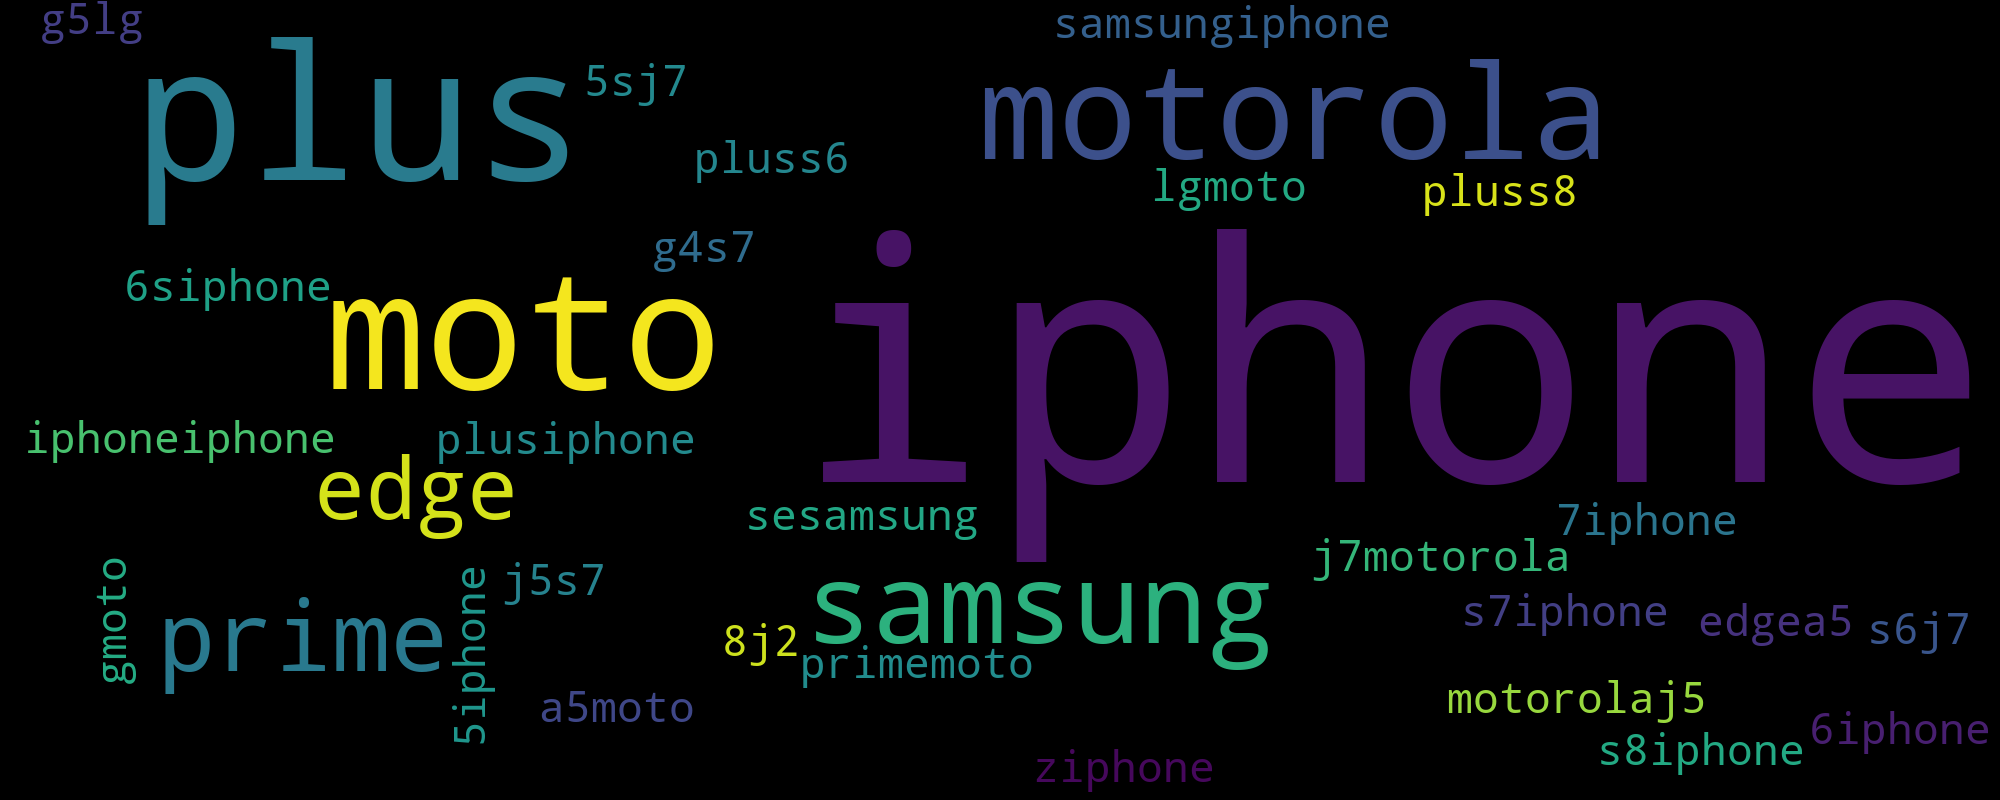
\includegraphics[width=\linewidth]{figures/07-search_terms-wordcloud.png}
	\caption{Términos más buscados por los usuarios de Trocafone}
	\label{searchedterm}
\end{figure}

Los términos más buscados son iPhone, Motorola y Samsung. Esto era completamente esperable debido a que son las marcas que dominan el sector tecnológico.

\subsection{Productos buscados en la plataforma}

En esta sección se busca obtener los productos más buscados. Esta búsqueda es más específica que la anteriormente mencionada debido a que corresponde a un producto puntual, no el nombre de su marca. De esta manera los productos más buscados son los que se detallan en la \texttt{Tabla 1} y se representan en el gráfico que le sigue.

Se concluye en esta sección que si bien \texttt{iPhone} y \texttt{Motorola} eran los términos más buscados en la plataforma, no sucede lo mismo con los productos buscados ya que todos corresponden a la marca \texttt{Samsung}. Esto puede deberse a un tema de la calidad que ofrece dicha marca o su precio, probablemente más conveniente. Los iPhone se caracterizan por tener un precio difícil de acceder por lo que es probable que sea buscado como término para ver las diferentes opciones globalmente pero que no muchas veces se busque un producto determinado de dicha marca.

\begin{table}[h!]
	\begin{center}
		\begin{tabular}{|l|l|}
			\hline
			sku & sku\_name \\
			\hline \hline
			3371 & Samsung Galaxy S6 Flat 32GB Dourado (Bom) \\ \hline			
			2777 & Samsung Galaxy S4 i9505 16GB Preto (Bom) \\ \hline
			6357 & Samsung Galaxy J5 16GB Preto (Bom) \\ \hline
			6413 & Samsung Galaxy J7 16GB Dourado (Bom) \\ \hline
			6371 & Samsung Galaxy J5 16GB Dourado (Bom) \\ \hline
		\end{tabular}
		\caption{SKUs más buscados y su nombre}
		\label{tabla:sencilla}
	\end{center}
\end{table}

\begin{figure}[h!]
	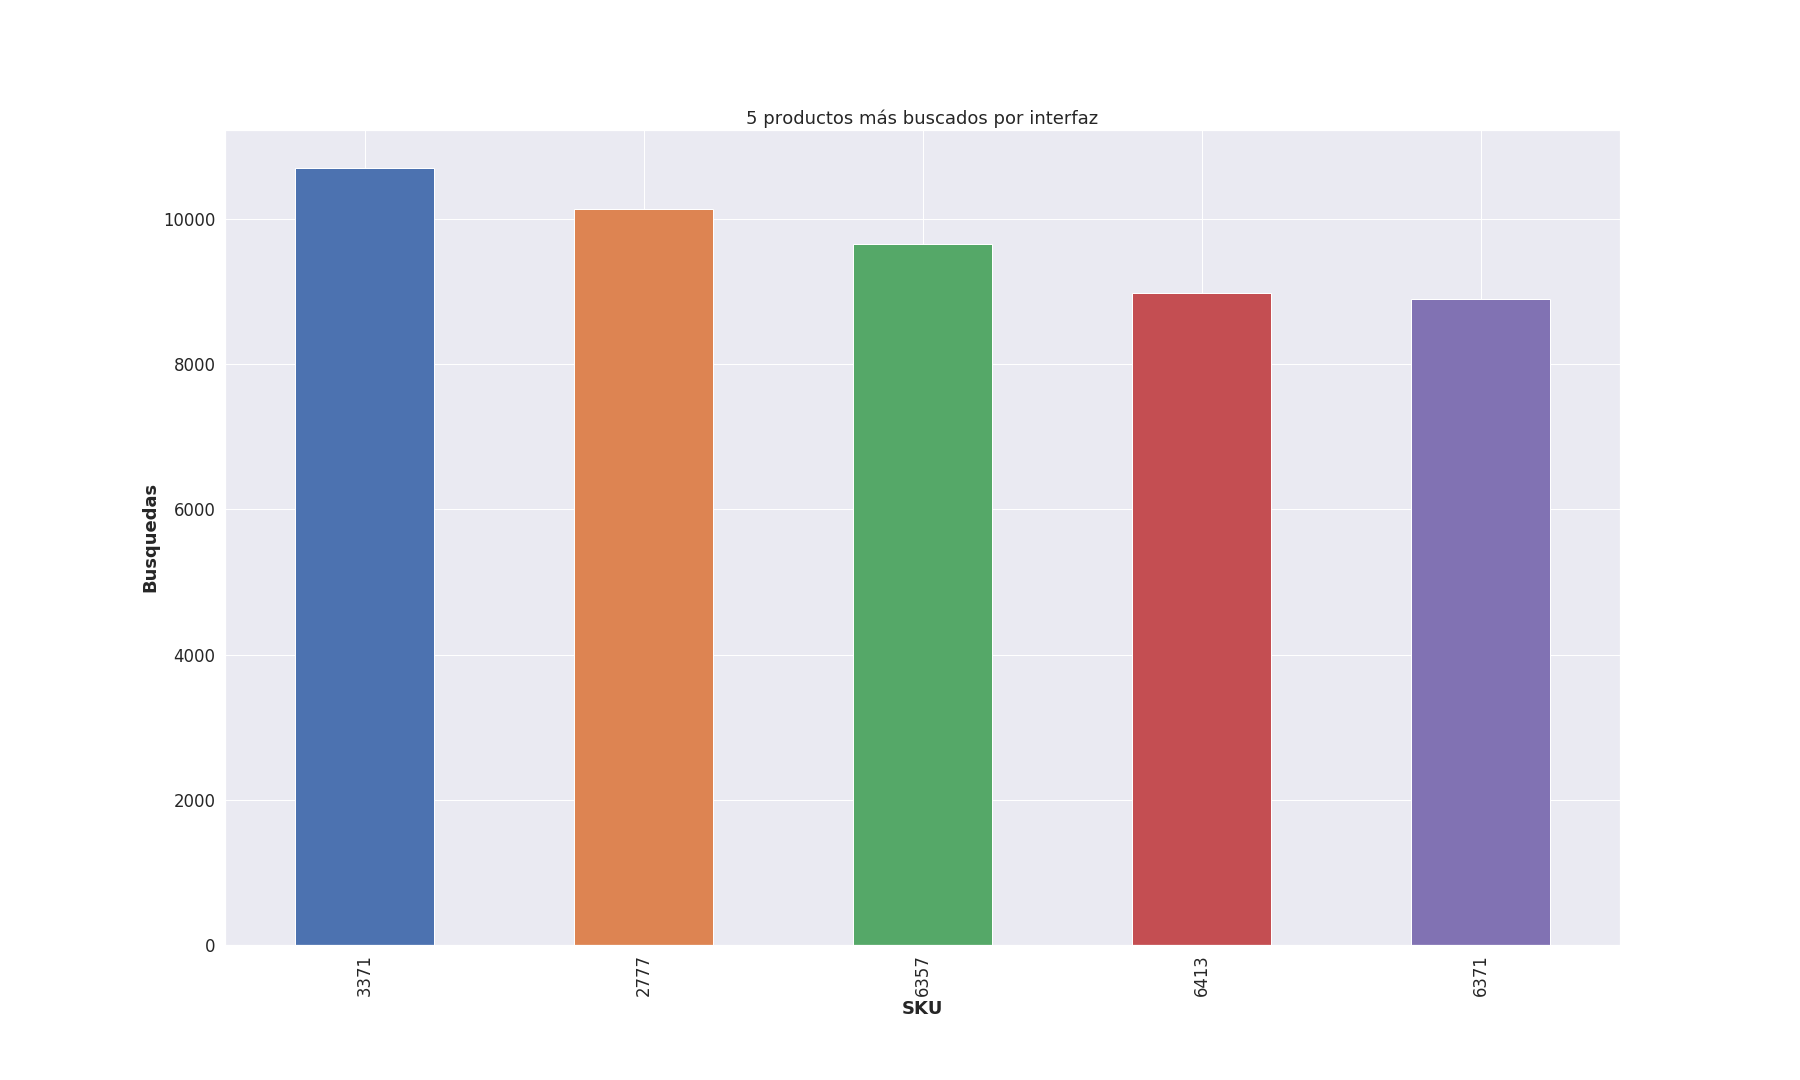
\includegraphics[width=\linewidth]{figures/08-skus_buscados-barplot.png}
	\caption{Productos más buscados por los usuarios de Trocafone}
	\label{searchedproduct}
\end{figure}

\section{Análisis de páginas estáticas}

Se propone comparar la cantidad de visitas al \texttt{FAQ} \footnote{Frequently Asked Questions: lista de preguntas y respuestas que surgen comúnmente en un contexto determinado.} con las de \texttt{Customer Service}.

La cantidad de visitas a \texttt{Customer Service} es mucho mayor que la cantidad de visitas al \texttt{FAQ}. Para mantener la página de \texttt{Customer Service} es necesario disponer de empleados constantemente para responder las consultas requeridas. Por lo tanto, se podría optimizar recursos redireccionando parte del tráfico a FAQ, haciendo más visibles los links a la página, agregando contenido común y mejorandola de ser necesario.

\begin{figure}[h!]
	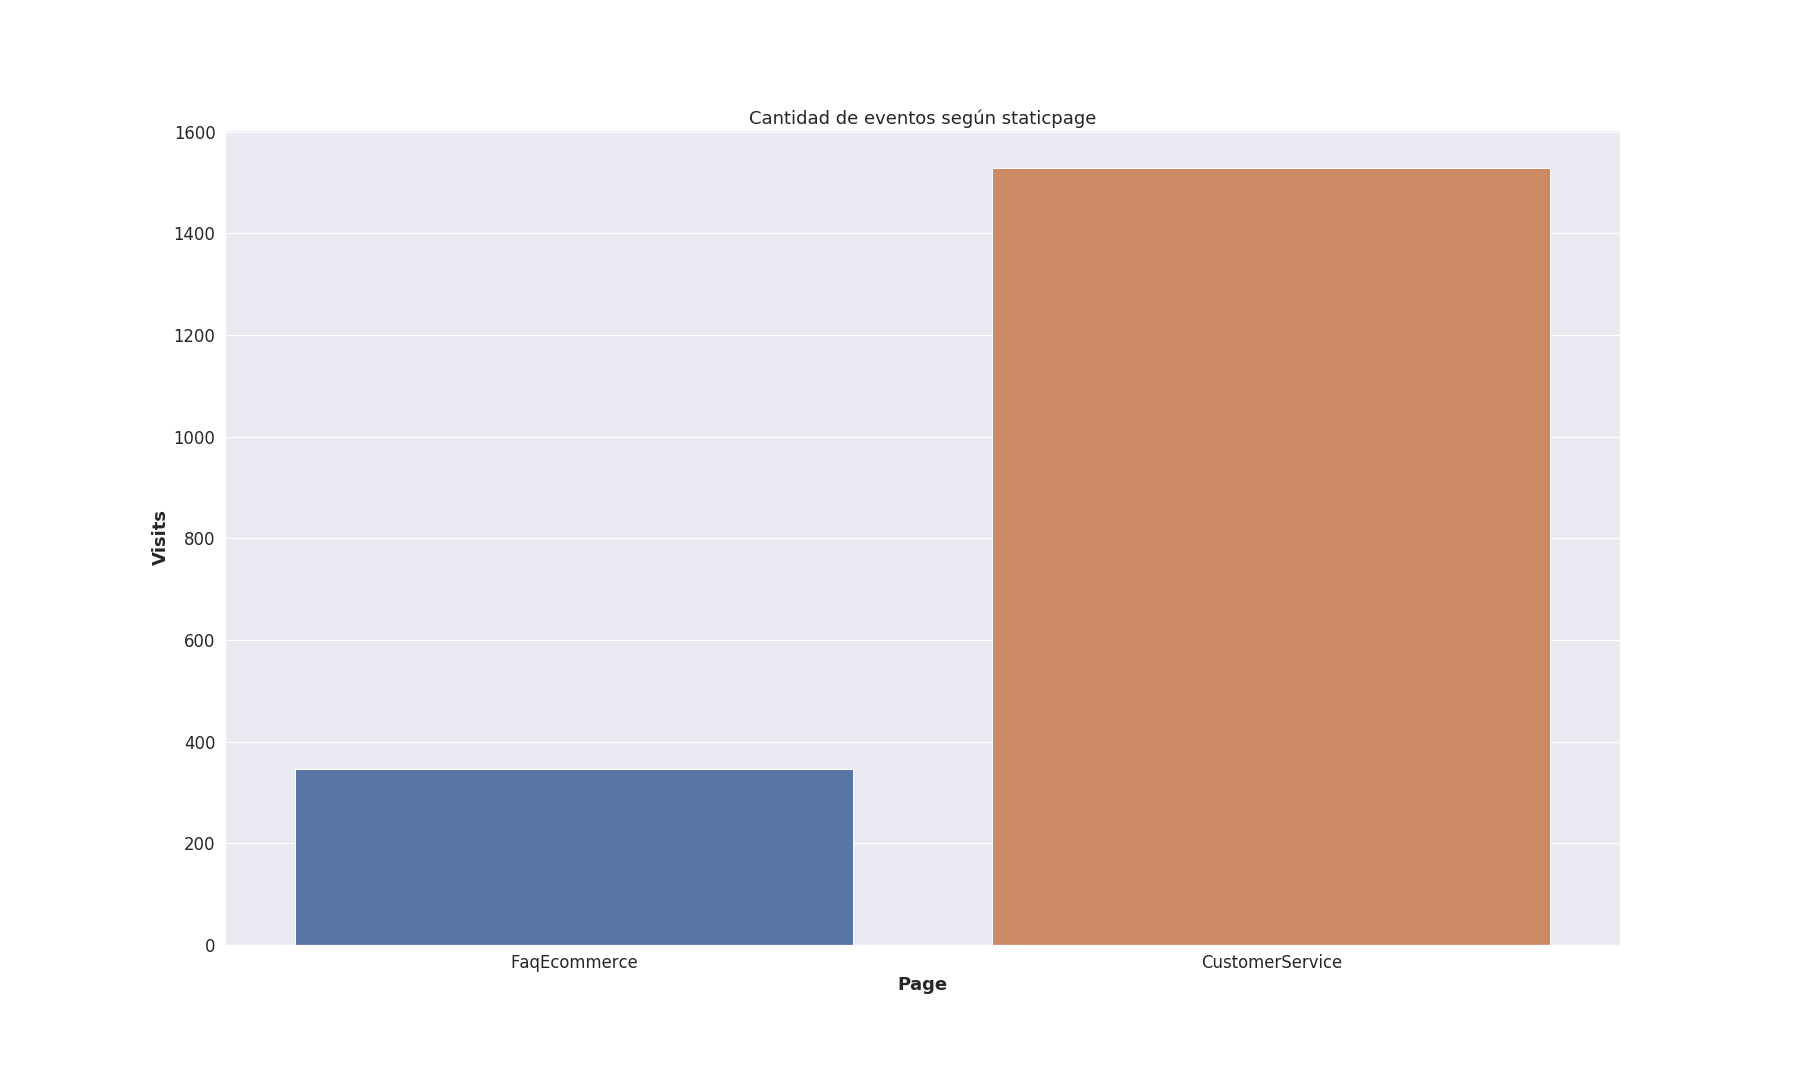
\includegraphics[width=11cm,height=11cm,keepaspectratio]{figures/12-static_pages-barplot.png}
	\caption{Comparación entre cantidad de visitas al FAQ y a Customer Service}
	\label{staticpage}
\end{figure}

\section{Análisis de New Vs Returning}

En esta sección se busca determinar la proporción de usuarios del sitio que entraron una sola vez a la página y no volvieron a hacerlo. Para ello se grafica en un primer lugar la cantidad de usuarios calificados como \texttt{New} contra los que son calificados como \texttt{Returning}.

\begin{figure}[h!]
	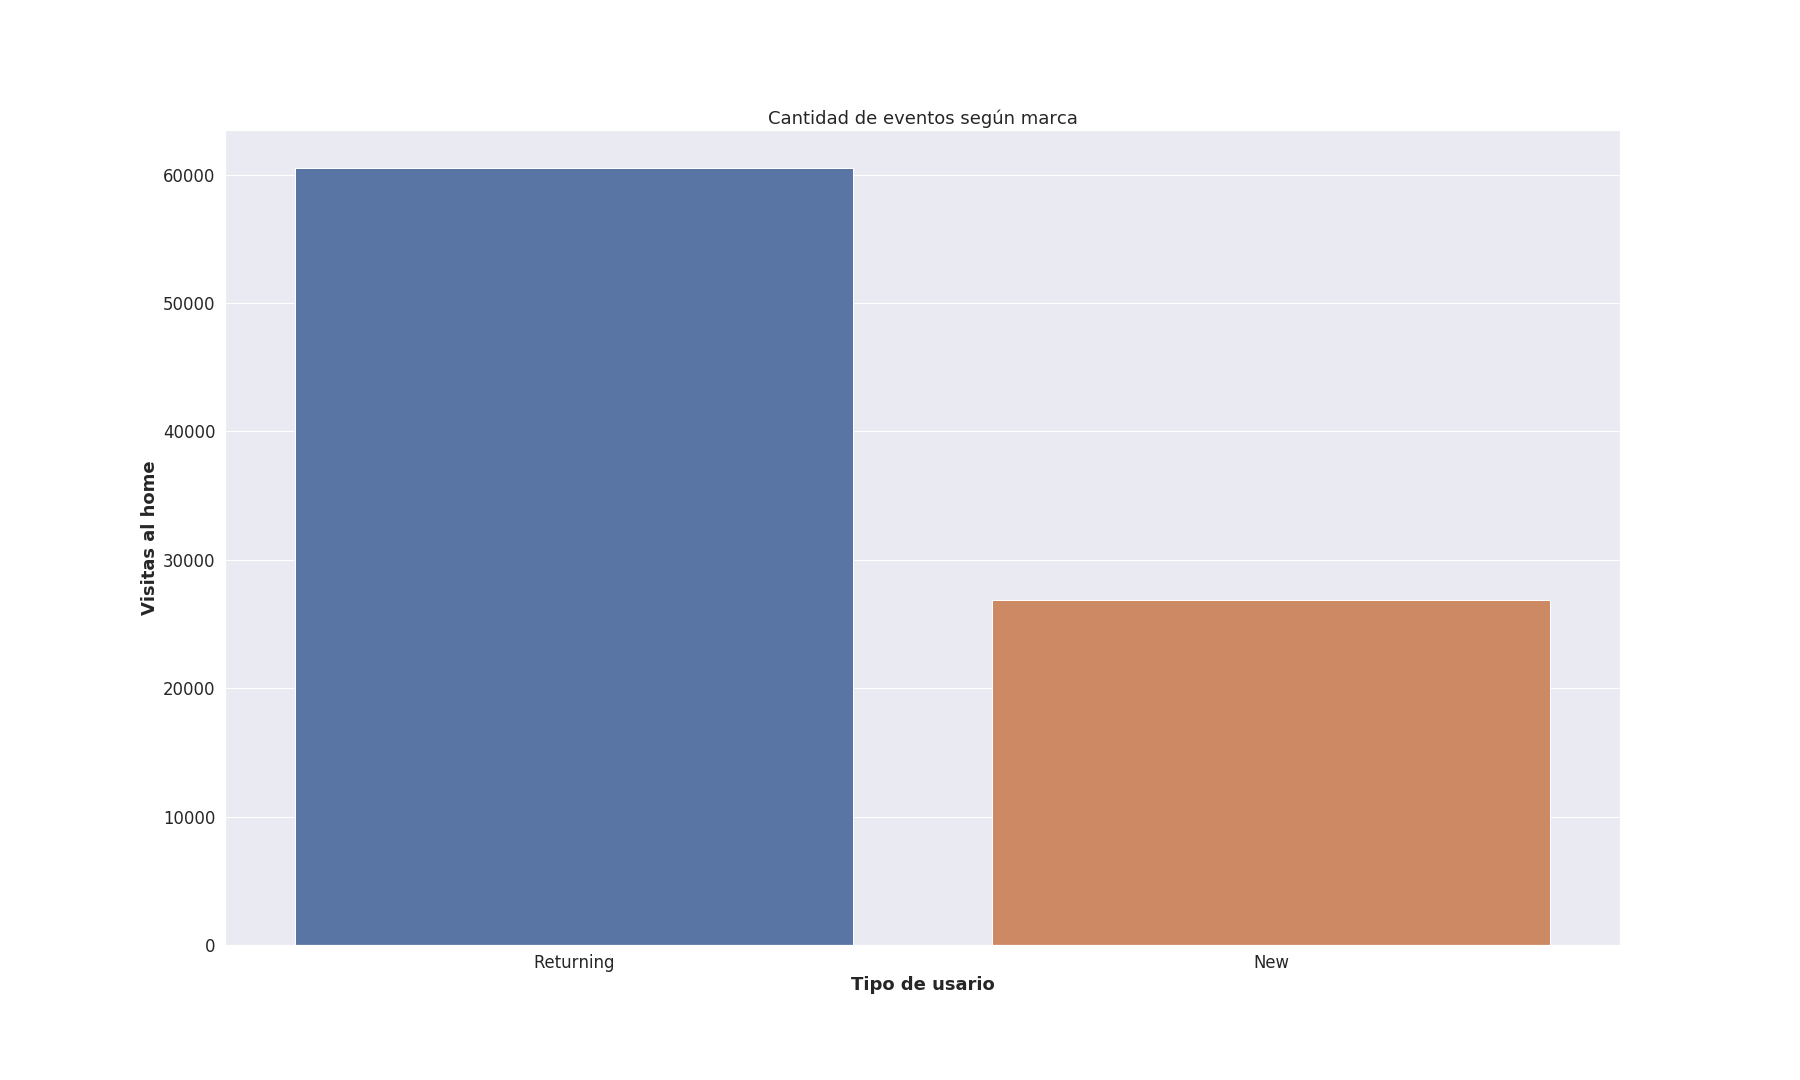
\includegraphics[width=11cm,height=11cm,keepaspectratio]{figures/130-eventos_new_returning-barplot.png}
	\caption{Comparación entre cantidad de usuarios que entran por primera vez al sitio contra los que volvieron}
	\label{newvsreturningfalse}
\end{figure}

Es necesario remarcar que este gráfico no es representativo porque todos los usuarios calificados como \texttt{returning} en algún momento fueron registrados como \texttt{new}. A simple vista se podría concluir que la proporción de usuarios que regresa es mucho mayor a los que entran solo 1 vez. 

Se realiza el recorte necesario para obtener una visualización que refleje fiablemente la cantidad de visitantes que entra al sitio 1 sola vez contra los que vuelven otras veces. 

\begin{figure}[h!]
	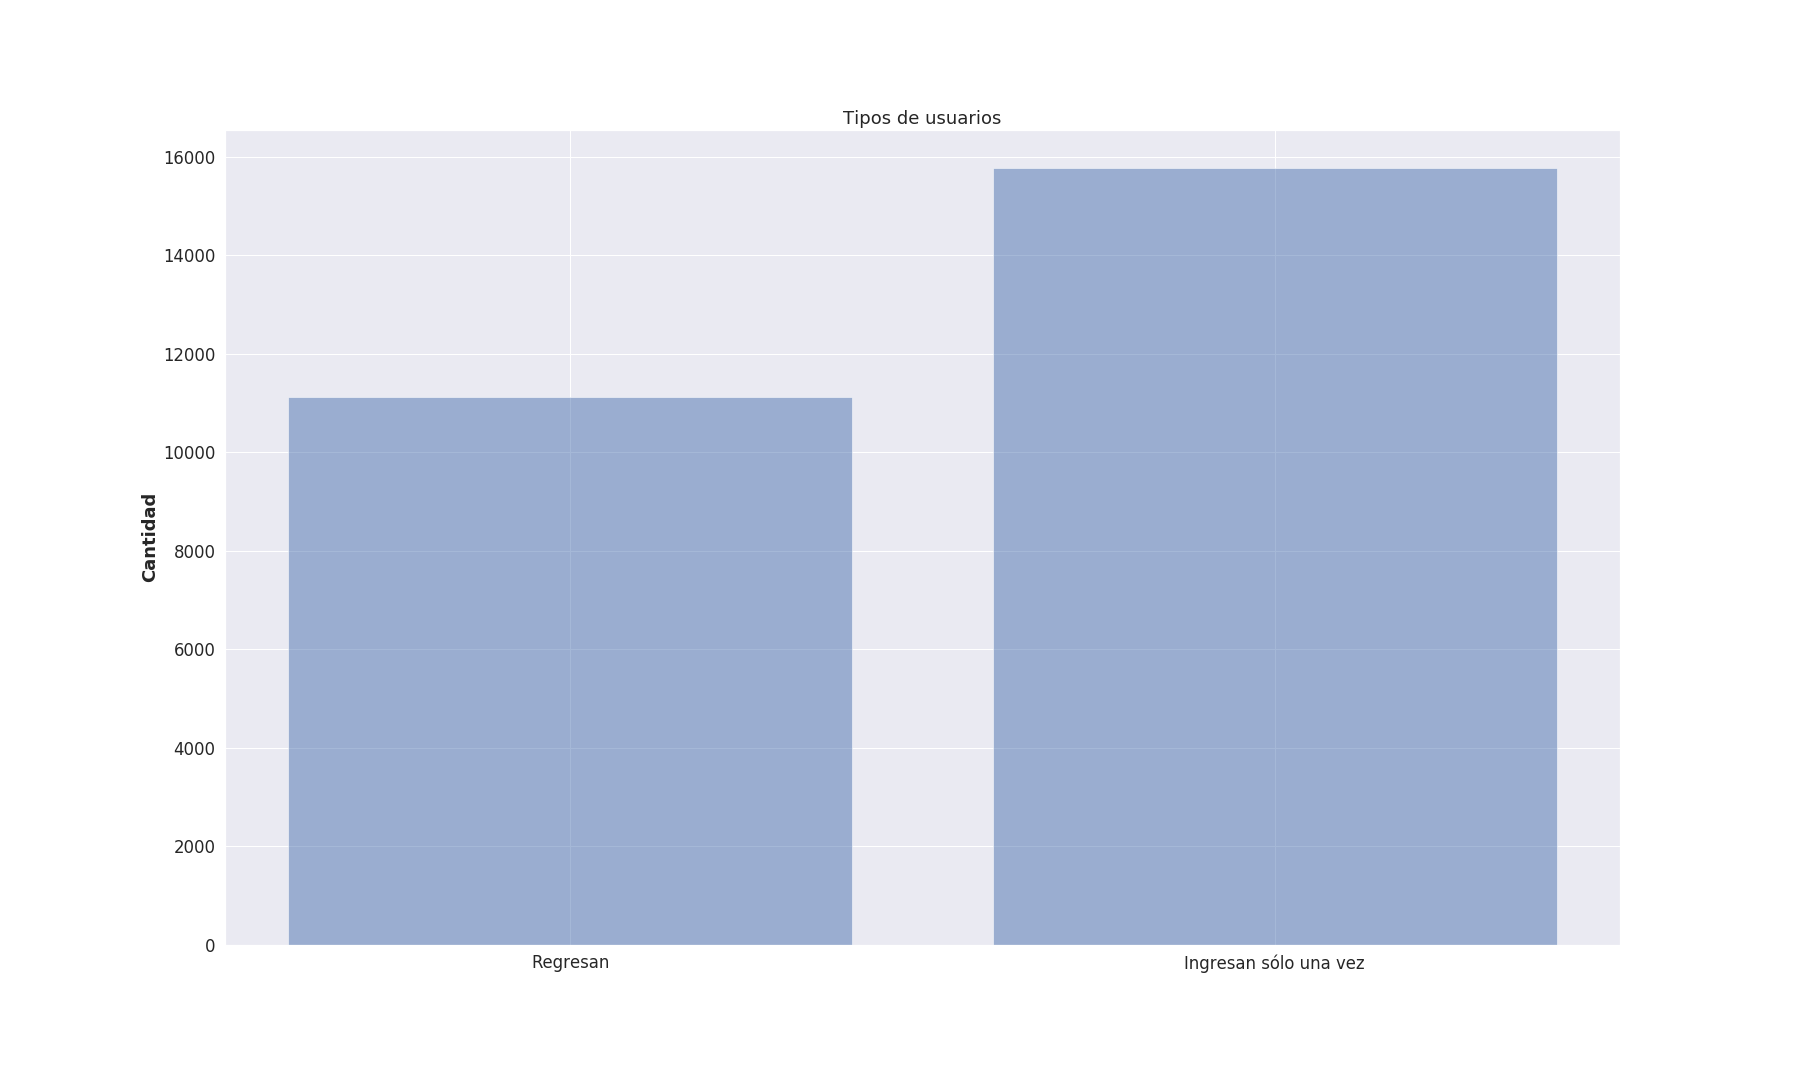
\includegraphics[width=11cm,height=11cm,keepaspectratio]{figures/131-tipos_usuarios-barplot.png}
	\caption{Comparación entre cantidad de usuarios que entran por primera vez al sitio contra los que volvieron}
	\label{newvsreturning}
\end{figure}

Se observa que la tasa de personas que entra una sola vez es mayor a la de las que regresan. Esta información desfavorece a Trocafone ya que implica que pierde una gran cantidad de clientes. Para aumentar la tasa de personas que regresan a ĺa página se puede proponer aumentar el presupuesto en publicidad y mejorar la experiencia de usuario de la home para que provea al usuario una experiencia más amena. También podrían ampliarse los métodos de pago o mejorar la página de \texttt{Customer Service} para que el cliente se sienta más contenido y pueda resolver todos los conflictos existentes ante una compra.

\end{document}